\chapter{Meta-learning Gaussian Process Property Predictors}
\label{chapter:adkf}

\ifpdf
    \graphicspath{{chapter0x-ADKF/figures}}
\else
    \graphicspath{}
\fi

This chapter presents an algorithm to fit parameters of
so-called ``deep kernel'' Gaussian processes
to multiple datasets in a meta-learning setting.
It was published as a conference paper
in ICLR 2023 \citep{chen2022meta}.
The conference paper was jointly written with
my supervisor José Miguel Hernández-Lobato
and fellow PhD student Wenlin Chen.
I had the original idea for the algorithm,
however Wenlin performed all experiments and wrote all code.
All three of us co-wrote the manuscript.

\section{Motivation}
\label{sec:adkf:motivation}

The latent space optimisation algorithm in Chapter~\ref{chapter:lso}
used a probabilistic model $h:\Z\mapsto\R$
to select latent vectors, which were then ``decoded'' by a generative model $g:\Z\mapsto\X$.
However, given an inverse ``encoder'' $q:\X\mapsto\Z$,
the composed function $h\circ q: \X\mapsto\R$
can be alternatively viewed as inducing predictions over $\X$ directly.
If $h$ is a Gaussian process (GP) model,
then this model is actually equivalent to a 
\emph{deep kernel Gaussian process}
\citep{hinton2007using,wilson2016deep,bradshaw2017adversarial,calandra2016manifold,ober21a}:
a prior over functions $f:\X\mapsto\R$
of the form
\begin{equation*}
    f\sim \mathcal{GP}\left(
        \bm{0},
        c_{\bftheta}\left(\nn_{\bfphi}(\cdot), \nn_{\bfphi}(\cdot)\right)
    \right)\ .
\end{equation*}
Here, 
$\nn_{\bfphi}:\X\mapsto\R^n$ is called the
\emph{feature extractor} (similar to $q$ from chapter~\ref{chapter:lso})
and $c_{\bftheta}:\R^n\times\R^n\mapsto\R$
is called the 
\emph{base kernel} (similar to $h$ from chapter~\ref{chapter:lso}).
The name ``deep kernel GP'' is appropriate because the GP's
kernel effectively contains a deep neural network.
The parameters of the feature extractor and base kernel
are denoted $\bftheta\in\Theta$
and $\bfphi\in\Phi$
respectively.
The set of all parameters in the deep kernel is denoted
$\bfpsi=(\bftheta,\bfphi)$.

Adopting this perspective reveals an important potential shortcoming of
weighted retraining method described in chapter~\ref{chapter:lso}:
that feature extractor parameters $\bfphi$ are selected based on a generative modelling
objective rather than a supervised learning objective
such as maximising the GP marginal likelihood
(equation~\ref{eqn:background:gp-marginal-likelihood}).
Presumably, incorporating a supervised learning objective
could improve the fit of the predictive model.
Unfortunately, \citet{ober21a} showed that deep kernel GPs
are highly susceptible to overfitting,
especially on smaller datasets.
This is highly problematic for molecule discovery, where most datasets are small
(sometimes fewer than 100 measurements).

However, between different tasks in molecule discovery
there are actually very many small datasets,
such that the total number of data points across all datasets is more sizeable.
This suggests that fitting deep kernel GPs in the meta-learning regime 
(\cref{sec:background:supervised learning}) may have the potential to avoid overfitting.
Therefore, this chapter presents a general method to efficiently fit deep kernel GPs in
meta-learning setting
called \emph{Adaptive Deep Kernel Fitting with Implicit Function Theorem} (ADKF-IFT).
ADKF-IFT essentially trains a subset of the model parameters with a meta-learning loss,
and separately adapts the remaining parameters on each task using maximum marginal likelihood.
In contrast to previous methods which use a single loss for all parameters,
ADKF-IFT is able to utilize the implicit regularization of meta-learning to prevent overfitting
while avoiding the strong assumptions of a pure meta-learning approach which may lead to underfitting.
    
    
\subsection{Notation for few-shot learning}

Following \citet{chen2022meta},
this chapter borrows some terminology from the few-shot learning literature \citep{miller2000learning,lake2011one}.
In particular, individual datasets are referred to as \emph{tasks}.

In the standard problem setup, one is given a set of training tasks $\dataset=\{\task_t\}_{t=1}^T$ (a \emph{meta-dataset})
and some unseen test tasks $\dataset_*=\{\task_*\}$.
Each task $\task=\{(\bfx_i, y_i)\}_{i=1}^{N_{\task}}$ is a set of points
in the domain $\domainx$ (e.g., space of molecules) with corresponding labels (continuous, categorical, etc.),
and is partitioned into a \emph{support set} $\support_{\task}\subseteq \task$ for training
and a \emph{query set} $\query_{\task}=\task \setminus \support_{\task}$ for testing.
Typically, the total number of training tasks $T=|\dataset|$ is large,
while the size of each support set $|\support_{\task}|$ is small.
Models for few-shot learning are typically trained to accurately predict $\query_{\task}$
given $\support_{\task}$
for $\task\in\dataset$ during a \emph{meta-training} phase,
then evaluated by their prediction error on $\query_{_{\task_*}}$ given $\support_{_{\task_*}}$
for unseen test tasks $\task_*\in\dataset_*$
during a \emph{meta-testing} phase.
        
\section{Adaptive Deep Kernel Fitting with Implicit Function Theorem}\label{sec:method}
    
    \subsection{The General ADKF-IFT Framework for Learning 
    Deep Kernel GPs}\label{ssec:general-ADKF-IFT}
    Let $A_{\Theta}$ and $A_{\Phi}$ respectively be the sets of base kernel and feature extractor parameters for a deep kernel GP.
    Denote the set of all parameters by $A_{\Psi} = A_{\Theta}\cup A_{\Phi}$.
    The key idea of the general ADKF-IFT framework is that only a subset of the parameters 
    ${\color{black}A_{\Psiml}}\subseteq A_{\Psi}$ will be {\color{black}adapted} to each individual task by minimising a train loss $\loss_T$,
    with the remaining set of parameters ${\color{black}A_{\Psimeta}}=A_{\Psi} \setminus {\color{black}A_{\Psiml}}$
    {\color{black}meta-learned} during a {\color{black}\emph{meta-training}} phase to yield the best possible validation loss $\loss_V$ \emph{on average} over many related training tasks (\emph{after} $A_{\Psiml}$ is separately adapted to each of these tasks).
    This can be naturally formalized as the following \emph{bilevel optimisation} problem:
    \begin{align}
        \psimeta^*\,=\,\,&\argmin_{\psimeta}~\mean_{p(\task)}[\loss_V(\psimeta, \psiml^*(\psimeta,\support_{\task} ),\task )],\label{eq:outer_loss}\\
        \mathrm{such\ that}\quad \psiml^*(\psimeta,\support_{\task} )\,=\,\,&\argmin_{\psiml}~\loss_T(\psimeta,\psiml,\support_{\task} ).\label{eq:inner_loss}
    \end{align}
    
    Equations~(\ref{eq:outer_loss}) and (\ref{eq:inner_loss}) are most easily understood by separately considering the meta-learned parameters
    $\psimeta$ and the task-specific parameters $\psiml$.
    For a given task $\task$ and an arbitrary value for the meta-learned parameters $\psimeta$, in Equation~(\ref{eq:inner_loss}) the task-specific parameters $\psiml$ are chosen to minimise the \emph{train loss} $\loss_T$ evaluated on the task's support set $\support_{\task}$.
    That is, $\psiml$ is \emph{adapted} to the support set $\support_{\task}$ of the task $\task$,
    with the aim of producing the best possible model on $\support_{\task}$ for the given value of $\psimeta$.
    The result is a model with optimal task-specific parameters $\psiml^*(\psimeta,\support_{\task})$ for the given meta-learned parameters $\psimeta$ and task $\task$.
    The remaining question is how to choose a value for the meta-learned parameters $\psimeta$,
    knowing that $\psiml$ will be adapted separately to each task.
    In Equation~(\ref{eq:outer_loss}),
    we propose to choose $\psimeta$ to minimise the expected \emph{validation loss} $\loss_V$ over a distribution of training tasks $p(\task)$.
    There are two reasons for this.
    First, on any given task $\task$, the validation loss
    usually reflects the performance metric of interest on the query set $\query_{\task}$ of $\task$
    (e.g., the prediction error).
    Second, because the same value of $\psimeta$ will be used for all tasks,
    it makes sense to choose a value whose \emph{expected performance} is good across many tasks drawn from $p(\task)$.
    That is, $\psimeta$ is chosen such that a GP achieves the lowest possible average validation loss on the query
    set $\query_{\task}$ of a random training task $\task\sim p(\task)$ after $\psiml$ is adapted to the task's support set $\support_{\task}$.
    
    In practice, $\psimeta$ would be optimised during a \emph{meta-training} phase using a set of
    training tasks $\dataset$ to approximate Equation~(\ref{eq:outer_loss}).
    After meta-training
    (i.e.,\@ at meta-test time),
    we make predictions for each unseen test task $\task_*$ using the joint GP posterior predictive distribution with optimal parameters $\psimeta^*$ and $\psiml^*(\psimeta^*,\support_{\task_*})$:
    \begin{align}
        p(\query_{_{\task_*}}^y|\query_{_{\task_*}}^{\bfx},\support_{_{\task_*}},\psimeta^*,\psiml^*(\psimeta^*,\support_{\task_*} )).\label{eq:test_pred}
    \end{align}
    
    Note that the description above does not specify a particular choice of
    $A_{\Psimeta}$, $A_{\Psiml}$, $\loss_T$, and $\loss_V$.
    This is intentional, as there are many reasonable choices for these quantities.
    Because of this, we believe that ADKF-IFT should be considered a \emph{general framework},
    with a particular choice for these
    being an \emph{instantiation} of the ADKF-IFT framework.
    We give examples of this in Sections~\ref{ssec:dkl-dkt-comparison} and \ref{sec:specific-implementation}.
    
    
    \subsection{Efficient Meta-Training Algorithm}\label{ssec:ift}
    
    In general, optimising bilevel optimisation objectives such as Equation~(\ref{eq:outer_loss}) is computationally complex,
    mainly because each evaluation of the objective requires solving a separate inner optimisation problem~(\ref{eq:inner_loss}).
    Although calculating the \emph{hypergradient} (i.e., total derivative) of the validation loss $\loss_V$ w.r.t. the meta-learned parameters $\psimeta$ would allow Equation~\plaineqref{eq:outer_loss} to be solved with gradient-based optimisation:
    \begin{align}
        \frac{d\loss_V}{d\psimeta}=\frac{\partial \loss_V}{\partial\psimeta}+\frac{\partial \loss_V}{\partial \psiml^*} \frac{\partial\psiml^*}{\partial\psimeta},\label{eq:hypergrad}
    \end{align}
    equation~\plaineqref{eq:hypergrad} reveals that this requires calculating $\nicefrac{\partial\psiml^*}{\partial\psimeta}$,
    i.e.,\@ how the optimal task-specific parameters $\psiml^*(\psimeta,\support_{\task})$ change with respect to the meta-learned parameters $\psimeta$.
    Calculating this naively with automatic differentiation platforms would require tracking the gradient through many iterations of the inner optimisation (\ref{eq:inner_loss}),
    which in practice requires too much memory to be feasible.
    Fortunately, because $\psiml^*$ is an optimum of the train loss $\loss_T$, Cauchy's \emph{Implicit Function Theorem} (IFT) provides a formula for calculating $\nicefrac{\partial\psiml^*}{\partial\psimeta}$ for an arbitrary value of the meta-learned parameters $\psimeta'$ and a given task $\task'$:
    \begin{align}
        \left.\frac{\partial\psiml^*
        }{\partial\psimeta}\right\vert_{\psimeta'} = \left.-\left( \frac{\partial^2\loss_T(\psimeta,\psiml,\support_{\task'} )}{\partial\psiml\partial\psiml^T} \right)^{-1}\frac{\partial^2\loss_T(\psimeta,\psiml,\support_{\task'} )}{\partial\psiml\partial\psimeta^T}\right\vert_{\psimeta',\psiml'},\label{eq:cauchy ift}
    \end{align}
    where $\psiml'=\psiml^*(\psimeta',\support_{\task'})$.
    The only potential problem with \Eqref{eq:cauchy ift}
    is the computation and inversion of the Hessian matrix $\displaystyle \frac{\partial^2\loss_T(\psimeta,\psiml,\support_{\task} )}{\partial\psiml\partial\psiml^T}$.
    This computation can be done exactly if $|A_{\Psiml}|$ is small, which is the case considered in this chapter (as will be discussed in Section \ref{sec:specific-implementation}).
    Otherwise, an approximation to the inverse Hessian (e.g., Neumann approximation \citep{lorraine20a,clarke2022scalable}) could be used, which reduces both the memory and computational complexities to $\mathcal{O}(|A_{\Psi}|)$.
    Combining Equations \plaineqref{eq:hypergrad} and \plaineqref{eq:cauchy ift}, we have a recipe for computing the hypergradient $\nicefrac{d\loss_V}{d\psimeta}$ exactly for a single task, as summarized in Algorithm \ref{alg:ADKF-IFT}. The meta-learned parameters $\psimeta$ can then be updated with the expected hypergradient over $p(\task)$.
    
    \begin{algorithm}[tbh]
    \small
    \caption{Exact hypergradient computation in ADKF-IFT.}\label{alg:ADKF-IFT}
    \begin{algorithmic}[1]
        \STATE \textbf{Input:} a training task $\task'$ and the current meta-learned parameters $\psimeta'$.
        \vspace{1ex}
        \STATE Solve Equation \plaineqref{eq:inner_loss} to obtain $\psiml'=\psiml^*(\psimeta',\support_{\task'})$.
        \STATE Compute $\bfg_1=\left.\frac{\partial \loss_V(\psimeta,\psiml,\task' )}{\partial\psimeta}\right\vert_{\psimeta',\psiml'}$ and $\bfg_2=\left.\frac{\partial \loss_V(\psimeta,\psiml,\task' )}{\partial \psiml}\right\vert_{\psimeta',\psiml'}$ by auto-diff.
        \STATE Compute the Hessian $\bfH=\left. \frac{\partial^2\loss_T(\psimeta,\psiml,\support_{\task'})}{\partial\psiml\partial\psiml^T}\right\vert_{\psimeta',\psiml'}$ by auto-diff.
        \STATE Solve the linear system $\bfv \bfH=\bfg_2$ for $\bfv$.
        \STATE Compute the mixed partial derivatives $\bfP=\left.\frac{\partial^2\loss_T(\psimeta,\psiml,\support_{\task'} )}{\partial\psiml\partial\psimeta^T}\right\vert_{\psimeta',\psiml'}$ by  auto-diff.
        \STATE \textbf{Output:} the hypergradient $\frac{d\loss_V}{d\psimeta}=\bfg_1-\bfv \bfP$. \hfill\COMMENT{Equations \plaineqref{eq:hypergrad} and \plaineqref{eq:cauchy ift}}
        \vspace{1ex}
    \end{algorithmic}
    \end{algorithm}
    
    
    \subsection{ADKF-IFT as a Unification of Previous Methods}\label{ssec:dkl-dkt-comparison}
    In prior work, the most common method used to train deep kernel GPs is to maximise the
    log marginal likelihood on a single dataset (optionally with extra regularization terms).
    This is commonly referred to as \emph{Deep Kernel Learning} (DKL) \citep{wilson2016deep}.
    Posing the problem as \emph{minimisation} instead of \emph{maximisation},
    DKL uses the loss
    \begin{equation}\label{eq:dkl-objective}
        \bfpsi^* = \argmin_{\bfpsi}\mathrm{NLML}\left(\bfpsi,\support_{\task}\right) 
    \end{equation}
    where 
    $\mathrm{NLML}(\bfpsi,\cdot)$ denotes the \emph{negative} log marginal likelihood 
    (equation~\ref{eqn:background:gp-marginal-likelihood})
    of a deep kernel GP with parameters $\bfpsi$ on the dataset $(\cdot)$.
    The most notable departure from DKL is \emph{Deep Kernel Transfer} (DKT) \citep{Patacchiola20},
    which instead proposes to train deep kernel GPs entirely using meta-learning,
    minimising the \emph{expected} NLML over a distribution of training tasks,
    namely
    \begin{equation}\label{eq:dkt-objective}
        \bfpsi^* = \argmin_{\bfpsi}\mean_{p(\task)}[\mathrm{NLML}(\bfpsi,\task)]
    \end{equation}
    
    Interestingly, both DKL and DKT can be viewed as \emph{special cases}
    of the general ADKF-IFT framework.
    It is simple to see that choosing the partition to be $A_{\Psimeta}=\varnothing$,  $A_{\Psiml}=A_{\Psi}$ and the train loss $\loss_T$ to be the NLML in Equations~\plaineqref{eq:outer_loss} and \plaineqref{eq:inner_loss} yields Equation~\plaineqref{eq:dkl-objective}:
    DKL is just ADKF-IFT if no parameters are meta-learned.
    Similarly, choosing the partition to be $A_{\Psimeta}=A_{\Psi}$, $A_{\Psiml}=\varnothing$
     and the validation loss $\loss_V$ to be the NLML in Equations~\plaineqref{eq:outer_loss} and \plaineqref{eq:inner_loss} yields Equation~\plaineqref{eq:dkt-objective}:
    DKT is just ADKF-IFT if all parameters are meta-learned.
    This makes ADKF-IFT \emph{strictly more general} than these two methods.

    
    \subsection[Highlighted ADKF-IFT Instantiation]{Highlighted ADKF-IFT Instantiation: Meta-learn $\bfphi$, Adapt $\bftheta$}\label{sec:specific-implementation}
    Among the many possible variations of ADKF-IFT,
    we wish to highlight the following instantation:
    \begin{itemize}
        \item $A_{\Psimeta}=A_\Phi$, i.e.,\@ all feature extractor parameters $\bfphi$ are meta-learned across tasks.
        \item $A_{\Psiml}=A_\Theta$, i.e.,\@ all base kernel parameters $\bftheta$ (e.g.,\@ noise, lengthscales, etc) are adapted.
        \item The train loss $\loss_T$ and validation loss $\loss_V$
        are the negative log GP marginal likelihood on $\support_{\task}$
        and the negative log joint GP predictive posterior on $\query_{\task}$ given $\support_{\task}$,
        respectively.
        Explicitly, the training loss equation is
        \begin{equation}
            \begin{split}
                \loss_T(\psimeta,\psiml,\support_{\task}) 
                &= -\log p(\support^y_{\task}|\support^{\bfx}_{\task},\psimeta,\psiml)\\
                &=\frac{1}{2}\left<\support^y_{\task} ,\bfK_{\support_{\task} }^{-1}\support^y_{\task} \right> + \frac{1}{2}\log\det (\bfK_{\support_{\task} }) + \frac{N_{\support_{\task} }}{2}\log(2\pi),\label{eq:train_loss}
            \end{split}
        \end{equation}
        where $\bfK_{\support_{\task} }=k_{\psimeta,\psiml}(\support^{\bfx}_{\task},\support^{\bfx}_{\task})+\sigma^2\bfI_{N_{\support_{\task}}}$.
        The validation loss equation is
        \begin{equation}
        \begin{split}
            \loss_V(\psimeta,\psiml,\task) 
            &= -\log p(\query^y_{\task}|\query^{\bfx}_{\task},\support_{\task},\psimeta,\psiml)\\
            &= -\log \calN(\query^y_{\task};\bfK_{\query_{\task}\support_{\task}}\bfK_{\support_{\task}}^{-1}\support^y_{\task}, \\
            &\qquad\qquad\ \  \bfK_{\query_{\task}}-\bfK_{\query_{\task}\support_{\task}}\bfK_{\support_{\task}}^{-1}\bfK_{\support_{\task}\query_{\task}}),\label{eq:val_loss}
        \end{split}
        \end{equation}
        where
        \begin{equation*}
            \bfK_{\query_{\task}}=k_{\psimeta,\psiml}(\query^{\bfx}_{\task},\query^{\bfx}_{\task})+\sigma^2\bfI_{N_{\query_{\task}}}\ ,
        \end{equation*}
        \begin{equation*}
            \bfK_{\support_{\task}\query_{\task}}=\bfK_{\query_{\task}\support_{\task}}^T=k_{\psimeta,\psiml}(\support_{\task}^{\bfx},\query_{\task}^{\bfx})\ ,
        \end{equation*}
        and $\mathcal N$ is the Gaussian probability density function.

    \end{itemize}
    
    There are several benefits to this choice.
    First,
    this particular choice of loss functions has the advantage that the prediction procedure during meta-testing (as defined in Equation \plaineqref{eq:test_pred})
    exactly matches the meta-training procedure,
    thereby closely following the principle of \emph{learning to learn}. 
    Second, 
    the partition of parameters can be intuitively understood as 
    meta-learning a generally useful feature extractor $\nn_{\bfphi}$
    such that it is possible on average to fit a low-loss GP to the feature representations extracted by $\nn_{\bfphi}$ for each individual task.
    This is very similar to previous transfer learning approaches.
    Third, 
    since most GP base kernels have only a handful of parameters,
    the Hessian in \Eqref{eq:cauchy ift} can be computed and inverted exactly
    during meta-training using Algorithm \ref{alg:ADKF-IFT};
    this removes any need for Hessian approximations.
    Fourth,
    the inner optimisation \plaineqref{eq:inner_loss} for $\psiml$ is computationally efficient,
    as it does not require backpropagating through the
    feature extractor $\nn_{\bfphi}$.
    
    More generally, we conjecture that adapting just the base kernel parameters will allow ADKF-IFT to achieve a better balance between overfitting and underfitting than either DKL or DKT.
    The relationship between these methods are visualized in Figure~\ref{fig:ADKF-IFT-illstration}.
    Panel (c) shows DKL, which trains a separate deep kernel GP for each task.
    It is not hard to imagine that this can lead to severe overfitting for small datasets,
    which has been observed empirically by \citet{ober21a}.
    Panel (b) shows DKT, which prevents overfitting by fitting one deep kernel GP for all tasks.
    However, this implicitly makes a strong assumption that all tasks come from an identical distribution over functions,
    including the same noise level, same amplitude, and same characteristic lengthscales, which is unlikely to hold in practice.\footnote{
        Different tasks might have different 
        output ranges and units for regression.
        For example, one task might have data in the range $1$-$20$ $\mu$M,
        while another might have $0$-$100\%$ inhibition, meaning that a single signal variance
        (kernel amplitude) will not model the data well.
    }
    Panel (a) shows ADKF-IFT, which allows these important parameters to be adapted, while still regularizing the feature extractor
    with meta-learning. We conjecture that adapting the base kernel parameters is more appropriate given the expected differences
    between tasks:
    two related tasks are more likely to have different noise levels
    or characteristic lengthscales than to require substantially different feature representations.
    
    \begin{figure}[htb]
        \centering
        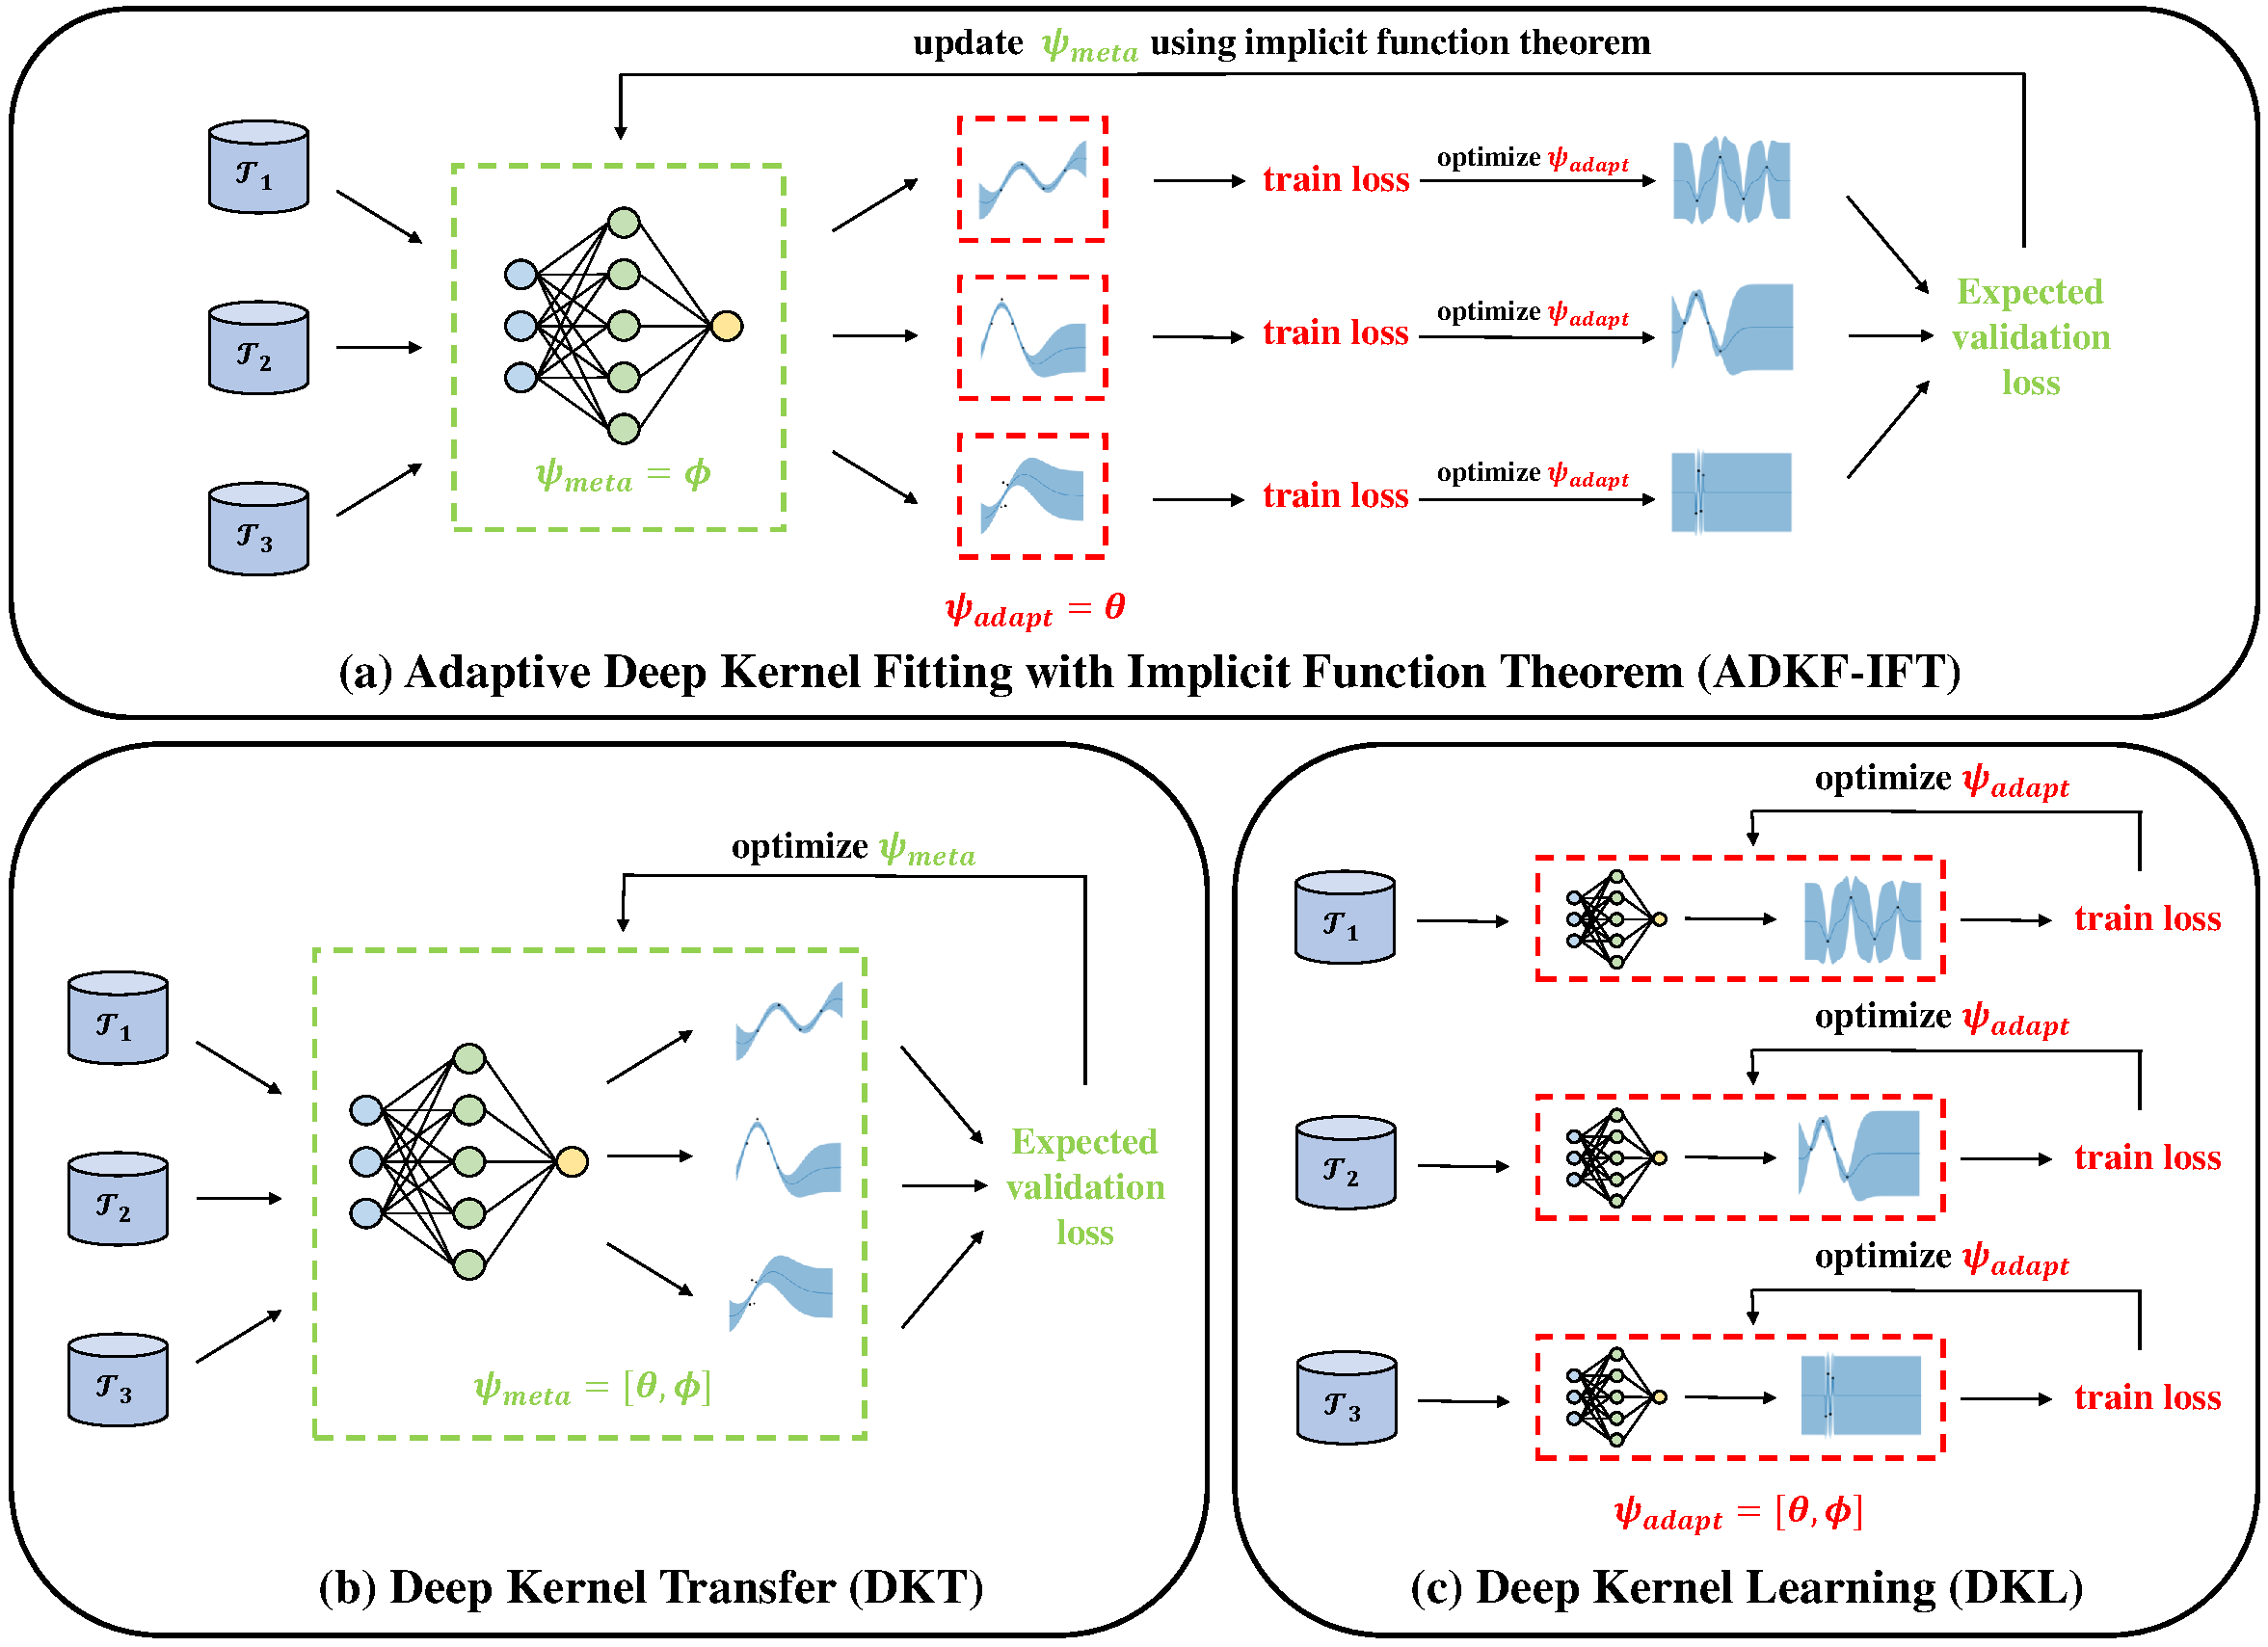
\includegraphics[width=0.9\textwidth]{illustration.pdf}
        \caption[Diagram illustrating the training procedures of ADKF-IFT, DKT, and DKL.]{
            Contrastive diagram illustrating the training procedures of ADKF-IFT, DKT, and DKL.
            (a) ADKF-IFT meta-learns some parameters and adapts others.
            (b) DKT meta-learns all parameters.
            (c) DKL adapts all parameters.
        }
        \label{fig:ADKF-IFT-illstration}
    \end{figure}

    Overall, ADKF-IFT combines DKL and DKT in a way that can potentially inherit the strengths of both methods
    and the weaknesses of neither.
    By adapting the base kernel parameters $\bftheta$ specifically to each task, it prevents underfitting due to varying ranges,
    lengthscales, or noise levels between datasets. By meta-learning the feature extractor on many datasets,
    it prevents overfitting as observed by \citet{ober21a}.
    

\section{Related Work}\label{sec:adkf:related-work}

    \subsection{Deep Kernel GPs}
    ADKF-IFT is part of a growing body of literature of techniques to train deep kernel GPs.
    As discussed in Section~\ref{ssec:dkl-dkt-comparison},
    ADKF-IFT \emph{generalizes} DKL \citep{wilson2016deep} and DKT \citep{Patacchiola20},
    which exclusively use single-task learning and meta-learning, respectively.
    \citet{liu2020simple} and \citet{van2021feature} propose adding regularization terms to the loss of DKL
    in order to mitigate overfitting.
    These works are better viewed as \emph{complementary} to ADKF-IFT rather than \emph{alternatives}:
    their respective regularization terms could easily be added to $\loss_T$ in Equation~\plaineqref{eq:inner_loss}
    to improve performance.
    However, the regularization strategies in both of these papers are designed for continuous inputs only,
    limiting their applicability to structured data like molecules.

    \subsection{Meta-learning}
    ADKF-IFT can also be viewed as a meta-learning algorithm
    comparable to many previously-proposed methods
    \citep{lake2011one,vinyals16,garnelo18a,triantafillou2019meta,Park2019meta,tian2020rethinking,chen2021self,liu2021meta,wistuba2021few,patacchiola2022contextual}.
    One distinguishing feature of ADKF-IFT is that it is specially designed for deep kernel GPs,
    whereas most methods from computer vision are designed exclusively for neural network models,
    which as previously stated are unsuitable when reliable uncertainty estimates are required.
    Furthermore, many of these algorithms such as ProtoNet \citep{snell2017prototypical} are designed principally or exclusively for classification,
    while ADKF-IFT is suited to both regression and classification.
    Compared to model-agnostic frameworks like MAML \citep{finn17a},
    ADKF-IFT does not require coarse approximations of the hypergradient due to its use of the implicit function theorem.

    \subsection{Multi-task Gaussian processes}
    ADKF-IFT can also be considered a method to learn multi-task GPs.
    The dominant approach to this problem in prior works is to learn a shared kernel for all data points across all tasks,
    transmitting information by explicitly modelling the covariance between data from different tasks
    \citep{kennedy2000predicting,forrester2007multi,bonilla2007multi,swersky2013multi,poloczek2017multi}.
    The main difference between methods in this family is the exact form of the kernel \citep{tighineanu2022transfer},
    which is typically assumed to have a particular structure (e.g.\@ Kronecker product or weighted sum of simpler kernels).
    ADKF-IFT cannot be naturally viewed in this way because the covariance
    between data points from separate tasks is always zero;
    information is instead transmitted between tasks via a shared set of
    kernel parameters.
    Therefore, we believe that ADKF-IFT is a significant departure from
    the dominant paradigm in GP transfer learning.
    
    \subsection{Implicit function theorem in machine learning}
    
    The implicit function theorem employed in our work has been used in many previous machine learning papers in various contexts, e.g., neural architecture search \citep{zhang2021idarts}, hyperparameter-tuning \citep{bengio2000gradient,luketina16,Pedregosa16hyper,lorraine20a,clarke2022scalable}, and meta-learning \citep{Rajeswaran2019iMAML,Lee_2019_CVPR,chen2020modular}.
    
    \subsection{Modular Meta-Learning with Shrinkage \citep{chen2020modular}}
    
    The method proposed by \citet{chen2020modular} shares many similarities
    with ADKF-IFT:
    at a high level it also divides model parameters
    into meta-learned and adapted parameters\footnote{
    They use the terms \emph{meta parameters} and \emph{task-specific parameters} instead.},
    and optimises the meta-learned parameters using the gradient of the validation
    loss after the adapted parameters have been adjusted to minimise the training loss
    using the implicit function theorem.
    The main differences between this work and ADKF-IFT are:
    \begin{enumerate}
        \item Model: \citet{chen2020modular} consider a model where $\phi$ are the means and variances of a Gaussian prior over model parameters,
        whereas in ADKF-IFT $\phi$ is a subset of the parameters of an arbitrary deep kernel GP.
        \item Hessian: \citet{chen2020modular} consider the case where $\Theta$ is too large to form the exact Hessian for the implicit function theorem. They instead use a conjugate gradient approximation.
        Although some instantiations of ADKF-IFT could require this,
        in our highlighted version the Hessian can be computed exactly,
        which we view as a significant advantage.
        \item Goal: The stated goal of \citet{chen2020modular} is to decide which parameters should be meta-learned,
        while in ADKF-IFT this must be pre-specified,
        and we give guidance for doing so in a way that results in transferable
        meta-learned features.
    \end{enumerate}

    \subsection{ADKL-GP \citep{tossou2019adaptive}}\label{ssec:adkl-explanation}
    
    The preprint of \citet{tossou2019adaptive} proposes an alternative adaptive deep kernel GP trained with meta-learning,
    where adaptation is performed by conditioning the feature extractor on an embedding of the entire support set
    rather than adjusting a subset of the kernel parameters as in ADKF-IFT.
    In general their empirical results were not very strong,
    and in our opinion the method is very prone to overfitting, which we explain below.
    
    The training objective for 
    ADKL-GP
    is equivalent to the objective for DKT
    with an added contrastive loss, weighted by a sensitive hyperparameter $\gamma$
    (see Equation (13) of \citet{tossou2019adaptive}).
    $\gamma$ can be interpreted as balancing the degree of regularization between two extremes:
    \begin{enumerate}
        \item If $\gamma=0$, there is no regularization of the task encoding network,
        making significant overfitting to the meta-dataset possible.
        This is effectively equivalent to standard DKL \citep{wilson2016deep}.
        \item As $\gamma\to\infty$,
        the regularization becomes infinitely strong,
        causing the task embeddings $\bfz_{\task}$ to collapse,
        and thereby preventing them from transmitting any information about specific datasets.
        With no information from $\bfz_{\task}$ in this case,
        the objective is essentially the same as that of DKT \citep{Patacchiola20}.
    \end{enumerate}
    For this method to be useful it would appear that $\gamma$ would need to be carefully tuned to balance between these extremes.
    \citet{tossou2019adaptive} perform a grid search over all hyperparameters including $\gamma\in\{0, 0.01, 0.1\}$
    but find no consistent trend besides $\gamma>0$ being slightly helpful,
    although the differences in performance were small.
    This suggests that the method may be difficult to use in practice.
    ADKF-IFT however has no such tunable hyperparameters,
    which we view as a significant strength.
    Instead, the balance between DKL and DKT is controlled by selecting which
    parameters are adapted and meta-learned,
    which is much more interpretable and makes it easier to use in practice.
    

\section{Experimental Evaluation on Molecules}\label{sec:adkf:experiments}

    In this section, we evaluate the empirical performance of ADKF-IFT from Section \ref{sec:specific-implementation}.
    We choose to focus our experiments exclusively on molecular property prediction and optimisation tasks
    because we believe this application would benefit greatly from better GP models:
    firstly because many existing methods struggle on small datasets of size $\sim 10^2$ which are ubiquitous in chemistry,
    and secondly because many tasks in chemistry require high-quality uncertainty estimates.
    First, we evaluate ADKF-IFT on four commonly used benchmark tasks from MoleculeNet \citep{wu2018moleculenet},
    finding that ADKF-IFT achieves state-of-the-art results on most tasks (Section~\ref{sec:few-shot-experiments-molnet}).
    Second, we evaluate ADKF-IFT on the larger-scale FS-Mol benchmark \citep{stanley2021fsmol},
    finding that ADKF-IFT is the best-performing method (Section~\ref{sec:few-shot-experiments}).
    In particular, our results support the hypothesis from Section~\ref{sec:specific-implementation}
    that ADKF-IFT achieves a better balance between overfitting and underfitting than DKL and DKT.
    Finally, we show that the ADKF-IFT feature representation is transferable to out-of-domain molecular property prediction and optimisation tasks (Section \ref{sec:adkf:mol-opt}).

    \subsection{Configuration of ADKF-IFT}

    All instances of ADKF-IFT use a GP model with a zero mean function and
    a Mat\'ern52 base kernel without automatic relevance determination (ARD) \citep{Neal1996-pm},
    since the typical sizes of the support sets in few-shot learning are too small to adjust a relatively
    large number of ARD lengthscales in ADKF-IFT.
    The lengthscale in the base kernel of ADKF-IFT is initialized using the median heuristic \citep{garreau2017large}
    for each task, with a log-normal prior centered at the initialization.
    Following \citet{Patacchiola20}, we treat binary classification as $\pm1$ label regression for ADKF-IFT.

    We solve the inner optimisation problem \plaineqref{eq:inner_loss} using the L-BFGS optimiser \citep{liu1989limited},
    since L-BFGS is the default choice for optimising base kernel parameters in the GP literature.
    For the outer optimisation problem \plaineqref{eq:outer_loss}, we approximate the expected hypergradient
    over $p(\task)$ by averaging the hypergradients for a batch of $K$ randomly sampled training tasks at each step,
    and update the meta-learned parameters $\psimeta$ with the averaged hypergradient using the Adam optimiser \citep{kingma2014adam}
    with learning rate $10^{-3}$ for MoleculeNet and $10^{-4}$ for FS-Mol. We set $K=10$ for MoleculeNet and $K=16$ for FS-Mol.
    For all experiments on FS-Mol, we evaluate the performance of our model on a small set of validation tasks during meta-training
    and use early stopping \citep{prechelt1998early} to avoid overfitting of $\psimeta$.
    
    \subsection{Few-shot Molecular Property Prediction on the MoleculeNet Benchmark}\label{sec:few-shot-experiments-molnet}
    
        \subsubsection{Benchmark and Baselines}
        We compare \textbf{ADKF-IFT} with two types of baselines on four few-shot molecular property
        classification benchmark tasks (Tox21, SIDER, MUV, and ToxCast) from MoleculeNet
        \citep{wu2018moleculenet}.
        The statistics of these datasets are summarized in Table~\ref{tab:molnet tasks}.

        \begin{table}[ht]
        \footnotesize
        \caption{Statistics of four few-shot molecular property prediction benchmarks from MoleculeNet.}
        \label{tab:molnet tasks}
        \centering
        \begin{tabular}{ccccc}
                \toprule
                \multirow{2}[3]{*}{Statistic} & \multicolumn{4}{c}{MoleculeNet benchmark task}\\
                \cmidrule(lr){2-5}
                & Tox21 & SIDER & MUV & ToxCast \\
                \midrule
                \#compounds & 8,014 & 1,427 & 93,127 & 8,615 \\
                \#tasks & 12 & 27 & 17 & 617  \\
                \#training tasks & 9 & 21 & 12 & 450  \\
                \#test tasks & 3 & 6 & 5 & 167 \\
                \bottomrule
            \end{tabular}
    \end{table}
        
        The first type of baseline is methods with feature extractor trained from scratch:
        \textbf{Siamese} \citep{Koch2015SiameseNN}, \textbf{ProtoNet} \citep{snell2017prototypical},
        \textbf{MAML} \citep{finn17a}, \textbf{TPN} \citep{liu2018learning},
        \textbf{EGNN} \citep{Kim2019EdgeLabelingGN}, \textbf{IterRefLSTM} \citep{AltaeTran2017LowDD} and
        \textbf{PAR} \citep{wang2021property}.
        The second type of baseline is methods which fine-tune a pretrained feature extractor:
        \textbf{Pre-GNN} \citep{Hu*2020Strategies}, \textbf{Meta-MGNN} \citep{guo2021few} and
        \textbf{Pre-PAR} \citep{wang2021property}.
        \textbf{Pre-ADKF-IFT} refers to ADKF-IFT starting from a pretrained feature extractor.
        All compared methods in this section use GIN \citep{Xu2019HowPA} as their feature extractors.
        The pretrained weights for the methods of the second type are provided by \citet{Hu*2020Strategies}.
        
        \subsubsection{Evaluation Procedure}
        We follow exactly the same evaluation procedure as that in \citet{wang2021property,Hu*2020Strategies,guo2021few}.
        The task-level metric is AUROC (area under the receiver operating characteristic curve).
        We report the averaged performance over ten runs with different random seeds for each compared method at the
        support set size 20 (i.e., $2$-way $10$-shot, as the support sets in MoleculeNet are balanced).
        We did not perform $1$-shot learning, as it is an unrealistic setting in real-world drug discovery tasks.
        All baseline results are taken from \citet{wang2021property}.
        
        \subsubsection{Performance}
        Table \ref{tab:molnet-results} shows that ADKF-IFT and Pre-ADKF-IFT achieve the best performance on
        Tox21, MUV, and ToxCast. In general, the larger the dataset is, the larger the performance gains
        of our method over other baselines are, highlighting the scalability of our method.
        The performance is lowest on SIDER (the smallest dataset),
        while it is highest on MUV (the largest dataset).

        While for most datasets the performance differences between methods are relatively small
        (within 10\%),
        the performance difference on MUV is particularly striking:
        it is near 100\% AUROC for ADKF-IFT and Pre-ADKF-IFT,
        while all other methods are below 70\%.
        The reason for this is unclear.
        \citet[page~6]{wu2024pacia} simply describe the result as an outlier.
        \citet[page~8]{wang2024knowledge} point to the
        fact that the MUV dataset has many unlabelled molecules and is extremely imbalanced
        as a possible cause.
        One possibility is that the positively labelled compounds tend to be very similar to each other,
        allowing methods which do some kind of nearest-neighbour comparison (like ADKF-IFT)
        to perform abnormally well.
        However, the large size of this dataset makes it difficult to validate this hypothesis.
        Ultimately, since MoleculeNet is an old benchmark with many known issues\footnote{
            These issue include data leakage in the train/test splits, presence of duplicate compounds,
            and inconsistent labels for many data points caused by aggregating heterogeneous data sources.
        }
        \citep{pat_walters_better_benchmarks},
        we do not believe that this result merits significant further analysis.
        
        \begin{table}
        \footnotesize
        \caption{Mean test performance (AUROC$\%$) with standard deviations of all compared methods on MoleculeNet benchmark tasks at support set size $20$ (i.e., $2$-way $10$-shot).}
        \label{tab:molnet-results}
            \centering
            \setlength\extrarowheight{-3pt}
            \begin{tabular}{ccccc}
                \toprule
                \multirow{2}[3]{*}{Method} & \multicolumn{4}{c}{MoleculeNet benchmark task (\#compounds)}\\
                \cmidrule(lr){2-5}
                & Tox21 (8,014) & SIDER (1,427) & MUV (93,127) & ToxCast (8,615) \\
                \midrule
                Siamese & $80.40\pm0.35$ & $71.10\pm4.32$ & $59.59\pm5.13$ & - \\
                ProtoNet & $74.98\pm0.32$ & $64.54\pm0.89$ & $65.88\pm4.11$ & $63.70\pm1.26$  \\
                MAML & $80.21\pm0.24$ & $70.43\pm0.76$ & $63.90\pm2.28$ & $66.79\pm0.85$ \\
                TPN & $76.05\pm0.24$ & $67.84\pm0.95$ & $65.22\pm5.82$ & $62.74\pm1.45$  \\
                EGNN & $81.21\pm0.16$ & $72.87\pm0.73$ & $65.20\pm2.08$ & $63.65\pm1.57$  \\
                IterRefLSTM & $81.10\pm0.17$ & $69.63\pm0.31$ & $45.56\pm5.12$ & -  \\
                PAR & $82.06\pm0.12$ & $\mathbf{74.68\pm0.31}$ & $66.48\pm2.12$ & $69.72\pm1.63$  \\
                ADKF-IFT & $\mathbf{82.43\pm0.60}$ & $67.72\pm1.21$ & $\mathbf{98.18\pm3.05}$ & $\mathbf{72.07\pm0.81}$  \\
                \midrule
                Pre-GNN & $82.14\pm0.08$ & $73.96\pm0.08$ & $67.14\pm1.58$ & $73.68\pm0.74$  \\
                Meta-MGNN & $82.97\pm0.10$ & $75.43\pm0.21$ & $68.99\pm1.84$ & -  \\
                Pre-PAR & $84.93\pm0.11$ & $\mathbf{78.08\pm0.16}$ & $69.96\pm1.37$ & $75.12\pm0.84$  \\ 
                Pre-ADKF-IFT & $\mathbf{86.06\pm0.35}$ & $70.95\pm0.60$ & $\mathbf{95.74\pm0.37}$ & $\mathbf{76.22\pm0.13}$  \\
                \bottomrule
            \end{tabular}
    \end{table}
    
    
    \subsection{Few-shot Molecular Property Prediction on the FS-Mol Benchmark}\label{sec:few-shot-experiments}
    
        \subsubsection{Benchmark}
        We further conduct our evaluation on the FS-Mol benchmark \citep{stanley2021fsmol},
        which contains a carefully constructed set of few-shot learning tasks for molecular property prediction.
        FS-Mol contains over 5,000 tasks with 233,786 unique compounds from ChEMBL27 \citep{mendez2019chembl},
        split into training (4,938 tasks), validation (40 tasks), and test (157 tasks) sets.
        Each task is associated with a protein target. The original benchmark only considers binary classification
        of active/inactive compounds, but we include the regression task (for the actual numeric activity target IC50 or EC50)
        in our evaluation as well, as it is a desired and more preferred task to do in real-world drug discovery projects. 
    
        \subsubsection{Baselines}
        We compare \textbf{ADKF-IFT} with four categories of baselines:
        \begin{enumerate}
            \item Single-task methods: Random Forest (\textbf{RF}), k-Nearest Neighbors (\textbf{kNN}),
                single-task GP with Tanimoto kernel (\textbf{GP-ST}) \citep{ralaivola2005graph}, single-task GNN
                (\textbf{GNN-ST}) \citep{gilmer2017neural}, Deep Kernel Learning (\textbf{DKL}) \citep{wilson2016deep}.

                These methods are trained separately on the
                support set of each test task, without leveraging the knowledge contained in the
                training tasks. The implementations of RF, kNN, and GNN-ST are taken from \citet{stanley2021fsmol}.
                RF, kNN, and GP-ST all operate on top of manually curated features obtained using 
                RF, kNN, and GP-ST represent molecules with count Morgan fingerprints with radius 2 and length 2048
                (\S\ref{definition:morgan-fingerprint})
                RF and kNN additionally concatenate a vector of 42 physicochemical descriptors
                calculated using RDKit.
                DKL operates on top of a combination of count Morgan fingerprints (also radius 2 and length 2048)
                and features extracted by a GNN.
                The base kernel used in DKL is the same as that used in ADKF-IFT.
                DKL is trained for 50 epochs on the support set of each test task.
                Hyperparameter search configurations for these methods are based on the
                extensive industrial experience from the authors of \citet{stanley2021fsmol}.
                GNN-ST uses a GNN with a hidden dimension of 128 and a gated readout function
                \citep{gilmer2017neural}, considering $\sim30$ hyperparameter search configurations.
            \item Multi-task pretraining: multi-task GNN (\textbf{GNN-MT}) \citep{corso2020principal,gilmer2017neural}.

                The implementation of GNN-MT is taken from \citet{stanley2021fsmol}.
                GNN-MT shares a GNN with a hidden dimension of 128 using principal neighbourhood
                message aggregation \citep{corso2020principal} across tasks, and uses a task-specific
                gated readout function \citep{gilmer2017neural} and an MLP with one hidden layer on top
                for each individual task. The model is trained on the support sets of all training
                tasks with early stopping based on the validation performance on the validation
                tasks. The task-specific components of the model are fine-tuned for each test task.
            \item Self-supervised pretraining: Molecule Attention Transformer (\textbf{MAT}) \citep{maziarka2020molecule}.

                The implementation of MAT is taken from \citet{stanley2021fsmol}.
                We use the official pretrained model parameters \citep{maziarka2020molecule},
                which is pretrained on 2 million molecules sampled from the ZINC15 dataset
                \citep{sterling2015zinc}. We fine-tuned it for each test task with hyperparameter
                search and early stopping based on 20\% of the support set for each task.   
            \item Meta-learning methods: {Property-Aware Relation Networks (\textbf{PAR})} \citep{wang2021property},
                Prototypical Network with Mahalanobis distance (\textbf{ProtoNet}) \citep{snell2017prototypical},
                Model-Agnostic Meta-Learning (\textbf{GNN-MAML}) \citep{finn17a}, Conditional Neural Process (\textbf{CNP})
                \citep{garnelo18a}, Deep Kernel Transfer (\textbf{DKT}) \citep{Patacchiola20}

                The implementations of ProtoNet and GNN-MAML are taken from \citet{stanley2021fsmol}.
                The implementation of {\color{black}PAR} is taken from its official implementation and
                integrated into the FS-Mol training and evaluation pipeline. PAR, ProtoNet, CNP, DKT, and
                ADKF-IFT operate on top of a combination of
                count Morgan fingerprints with radius 2 and size 2048 (\S\ref{definition:morgan-fingerprint}, same as above)
                and features extracted by a GNN. The GNN feature extractor architecture used for DKL,
                {PAR}, CNP, DKT, and ADKF-IFT is the same as that used for ProtoNet,
                GNN-MAML, GNN-ST, and GNN-MT in \citet{stanley2021fsmol}, with the size of the feature
                representation being tuned on the validation tasks. The base kernel used in DKT is the
                same as that used in ADKF-IFT.
        \end{enumerate}
        The GNN feature extractor architecture $\nn_{\bfphi}$ used for DKL, {\color{black}PAR}, CNP, DKT, and ADKF-IFT
        is the same as that used for ProtoNet, GNN-ST, GNN-MT, and GNN-MAML in \citet{stanley2021fsmol}. 
        All multi-task and meta-learning methods are trained from scratch on FS-Mol training tasks.
        MAT is pretrained on 2 million molecules sampled from the ZINC15 dataset \citep{sterling2015zinc}.
        The classification results for RF, kNN, GNN-ST, GNN-MT, MAT, ProtoNet, and GNN-MAML are reproduced according to
        \citet{stanley2021fsmol}.
        
        \subsubsection{Evaluation Procedure}
        Following \citet{stanley2021fsmol},
        the task-level metrics for binary classification and regression are $\Delta$AUPRC
        (change in area under the
        precision-recall curve) and $R^2_{os}$ (predictive/out-of-sample coefficient of determination),
        respectively.
        We follow exactly the same evaluation procedure as that in \citet{stanley2021fsmol},
        where the averaged performance over ten different stratified support/query random splits of every test task 
        s reported for each compared method. This evaluation process is performed for five different
        support set sizes 16, 32, 64, 128, and 256. Note that the support sets are generally
        unbalanced for the classification task in FS-Mol, which is natural as the majority of the
        candidate molecules are inactive in drug discovery.

        
        \subsubsection{Overall Performance}
        \begin{figure}
            \begin{subfigure}{.45\textwidth}
                \centering
                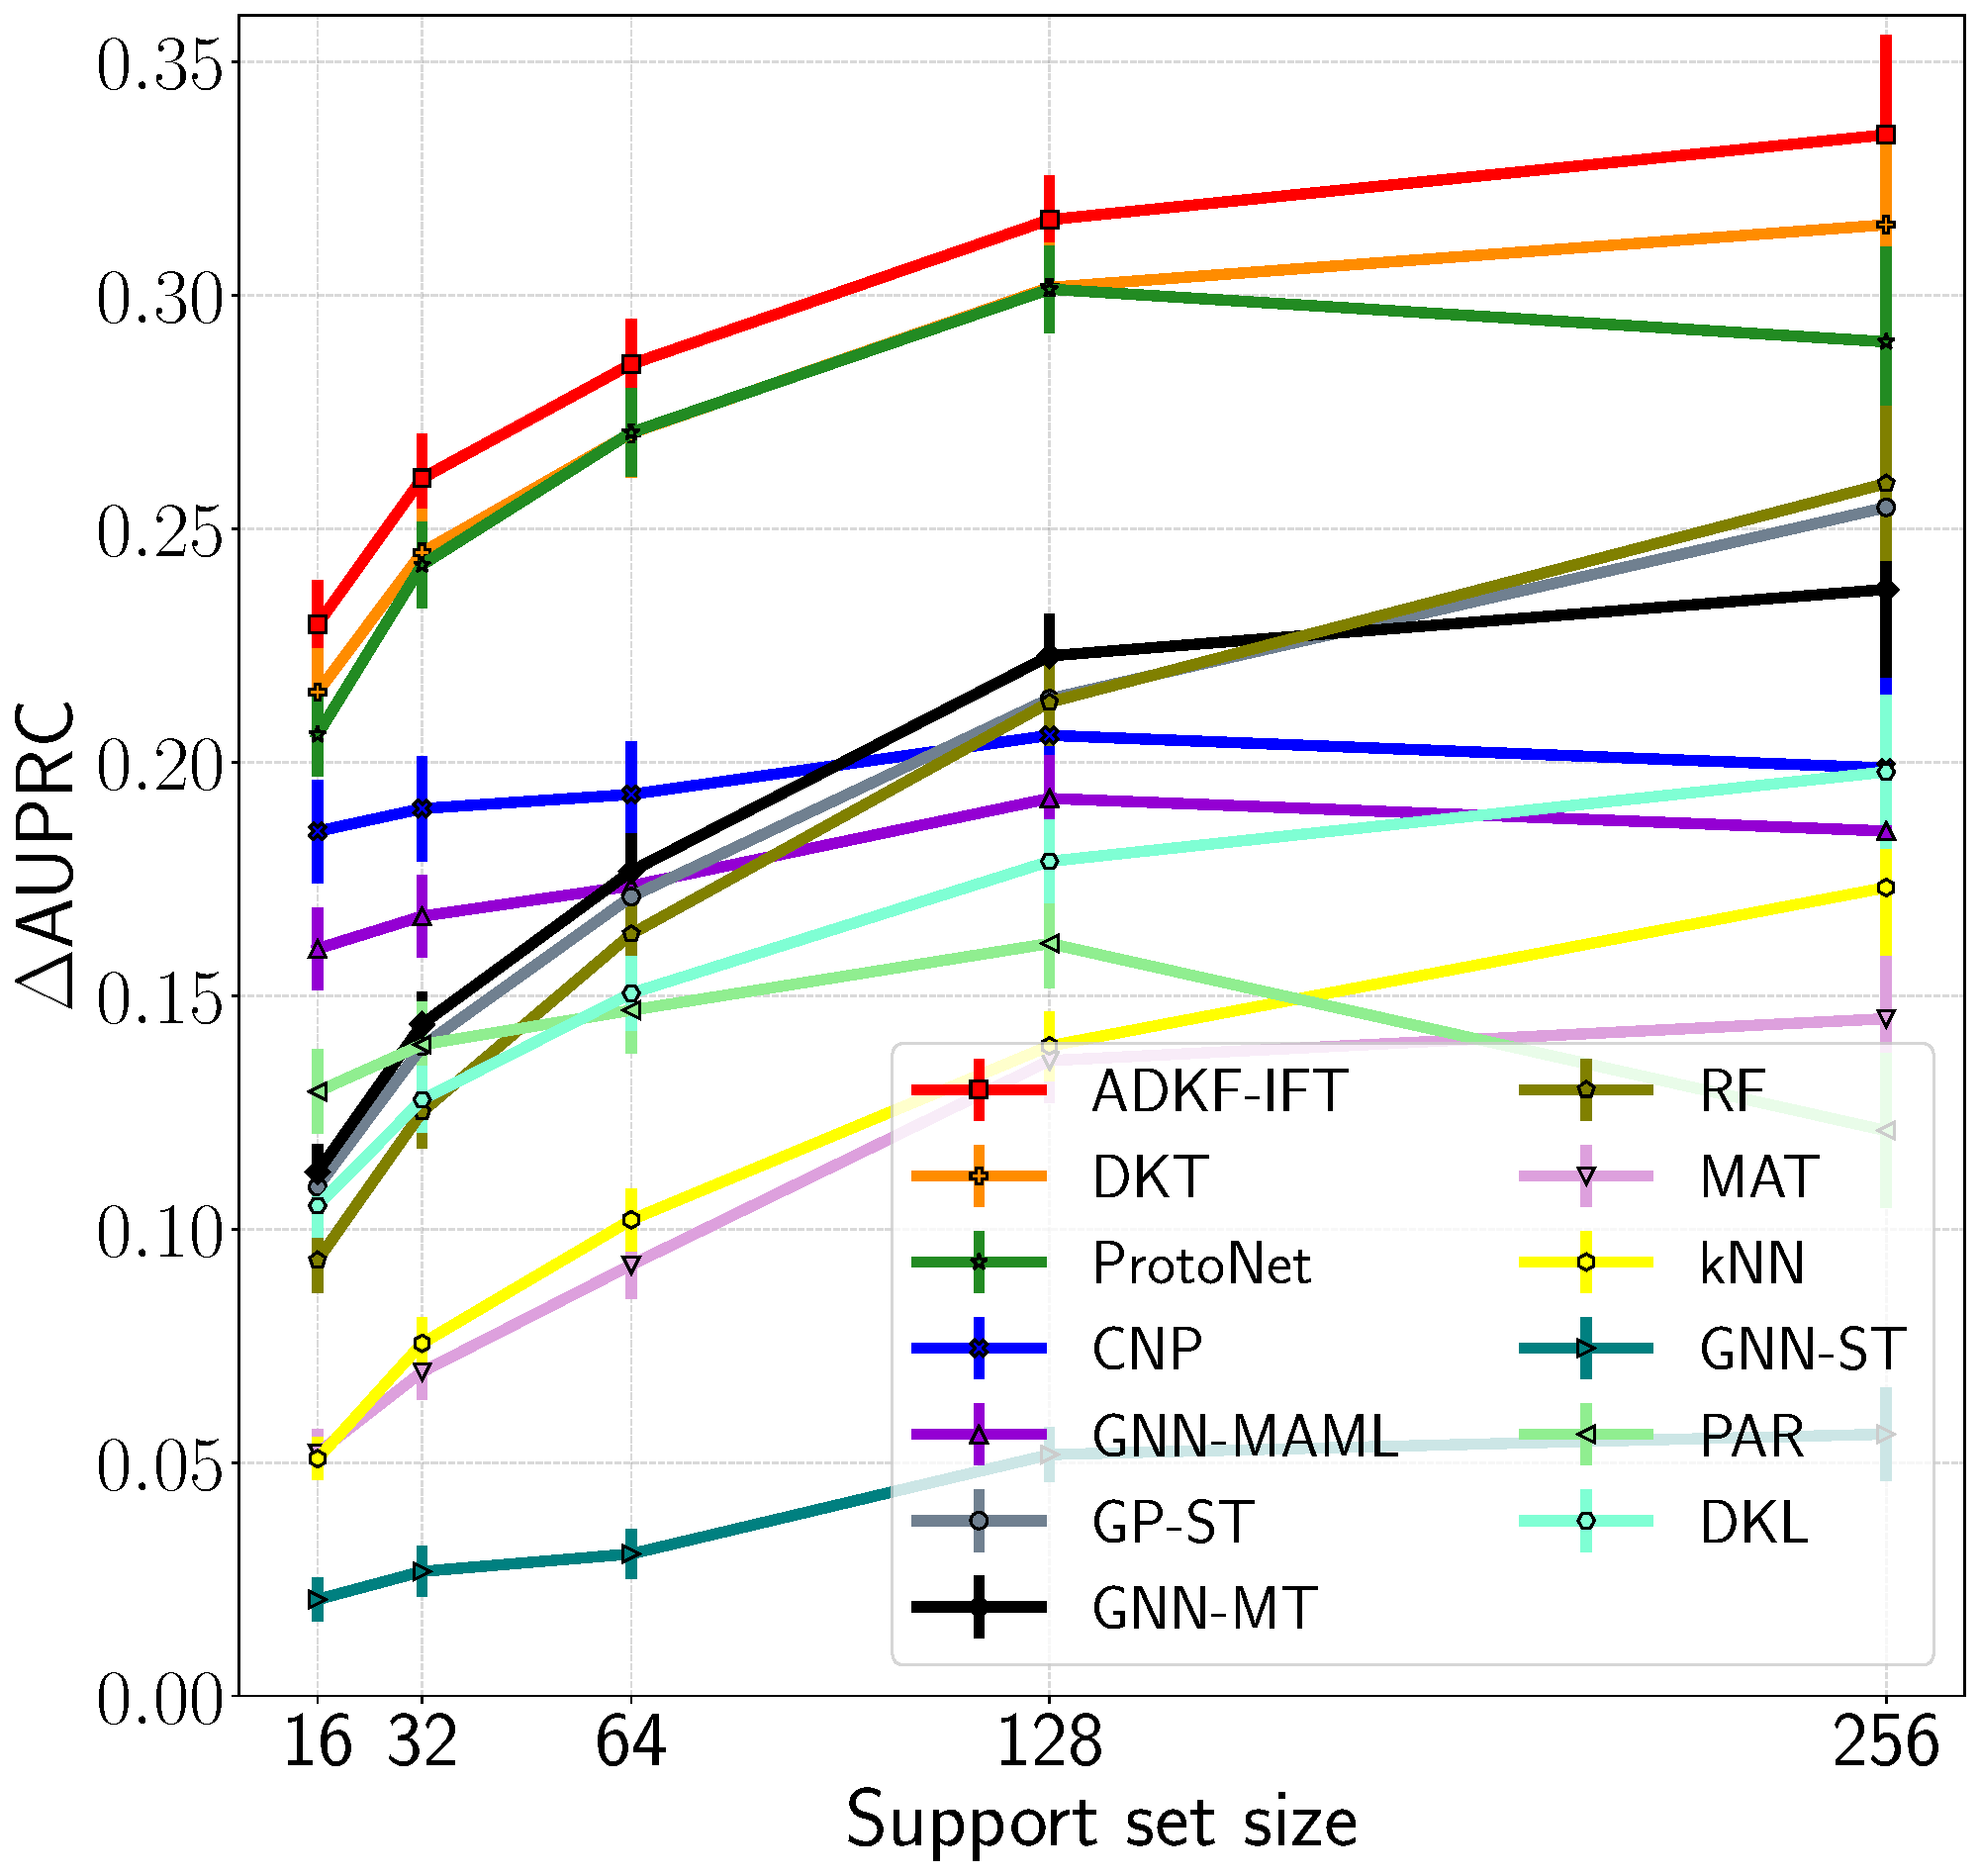
\includegraphics[width=\textwidth]{comparison_plot_hc_all.pdf}
                \caption{{\color{black}Classification (157 tasks).}}
            \end{subfigure}
            \hfill
            \begin{subfigure}{.45\textwidth}
                \centering
                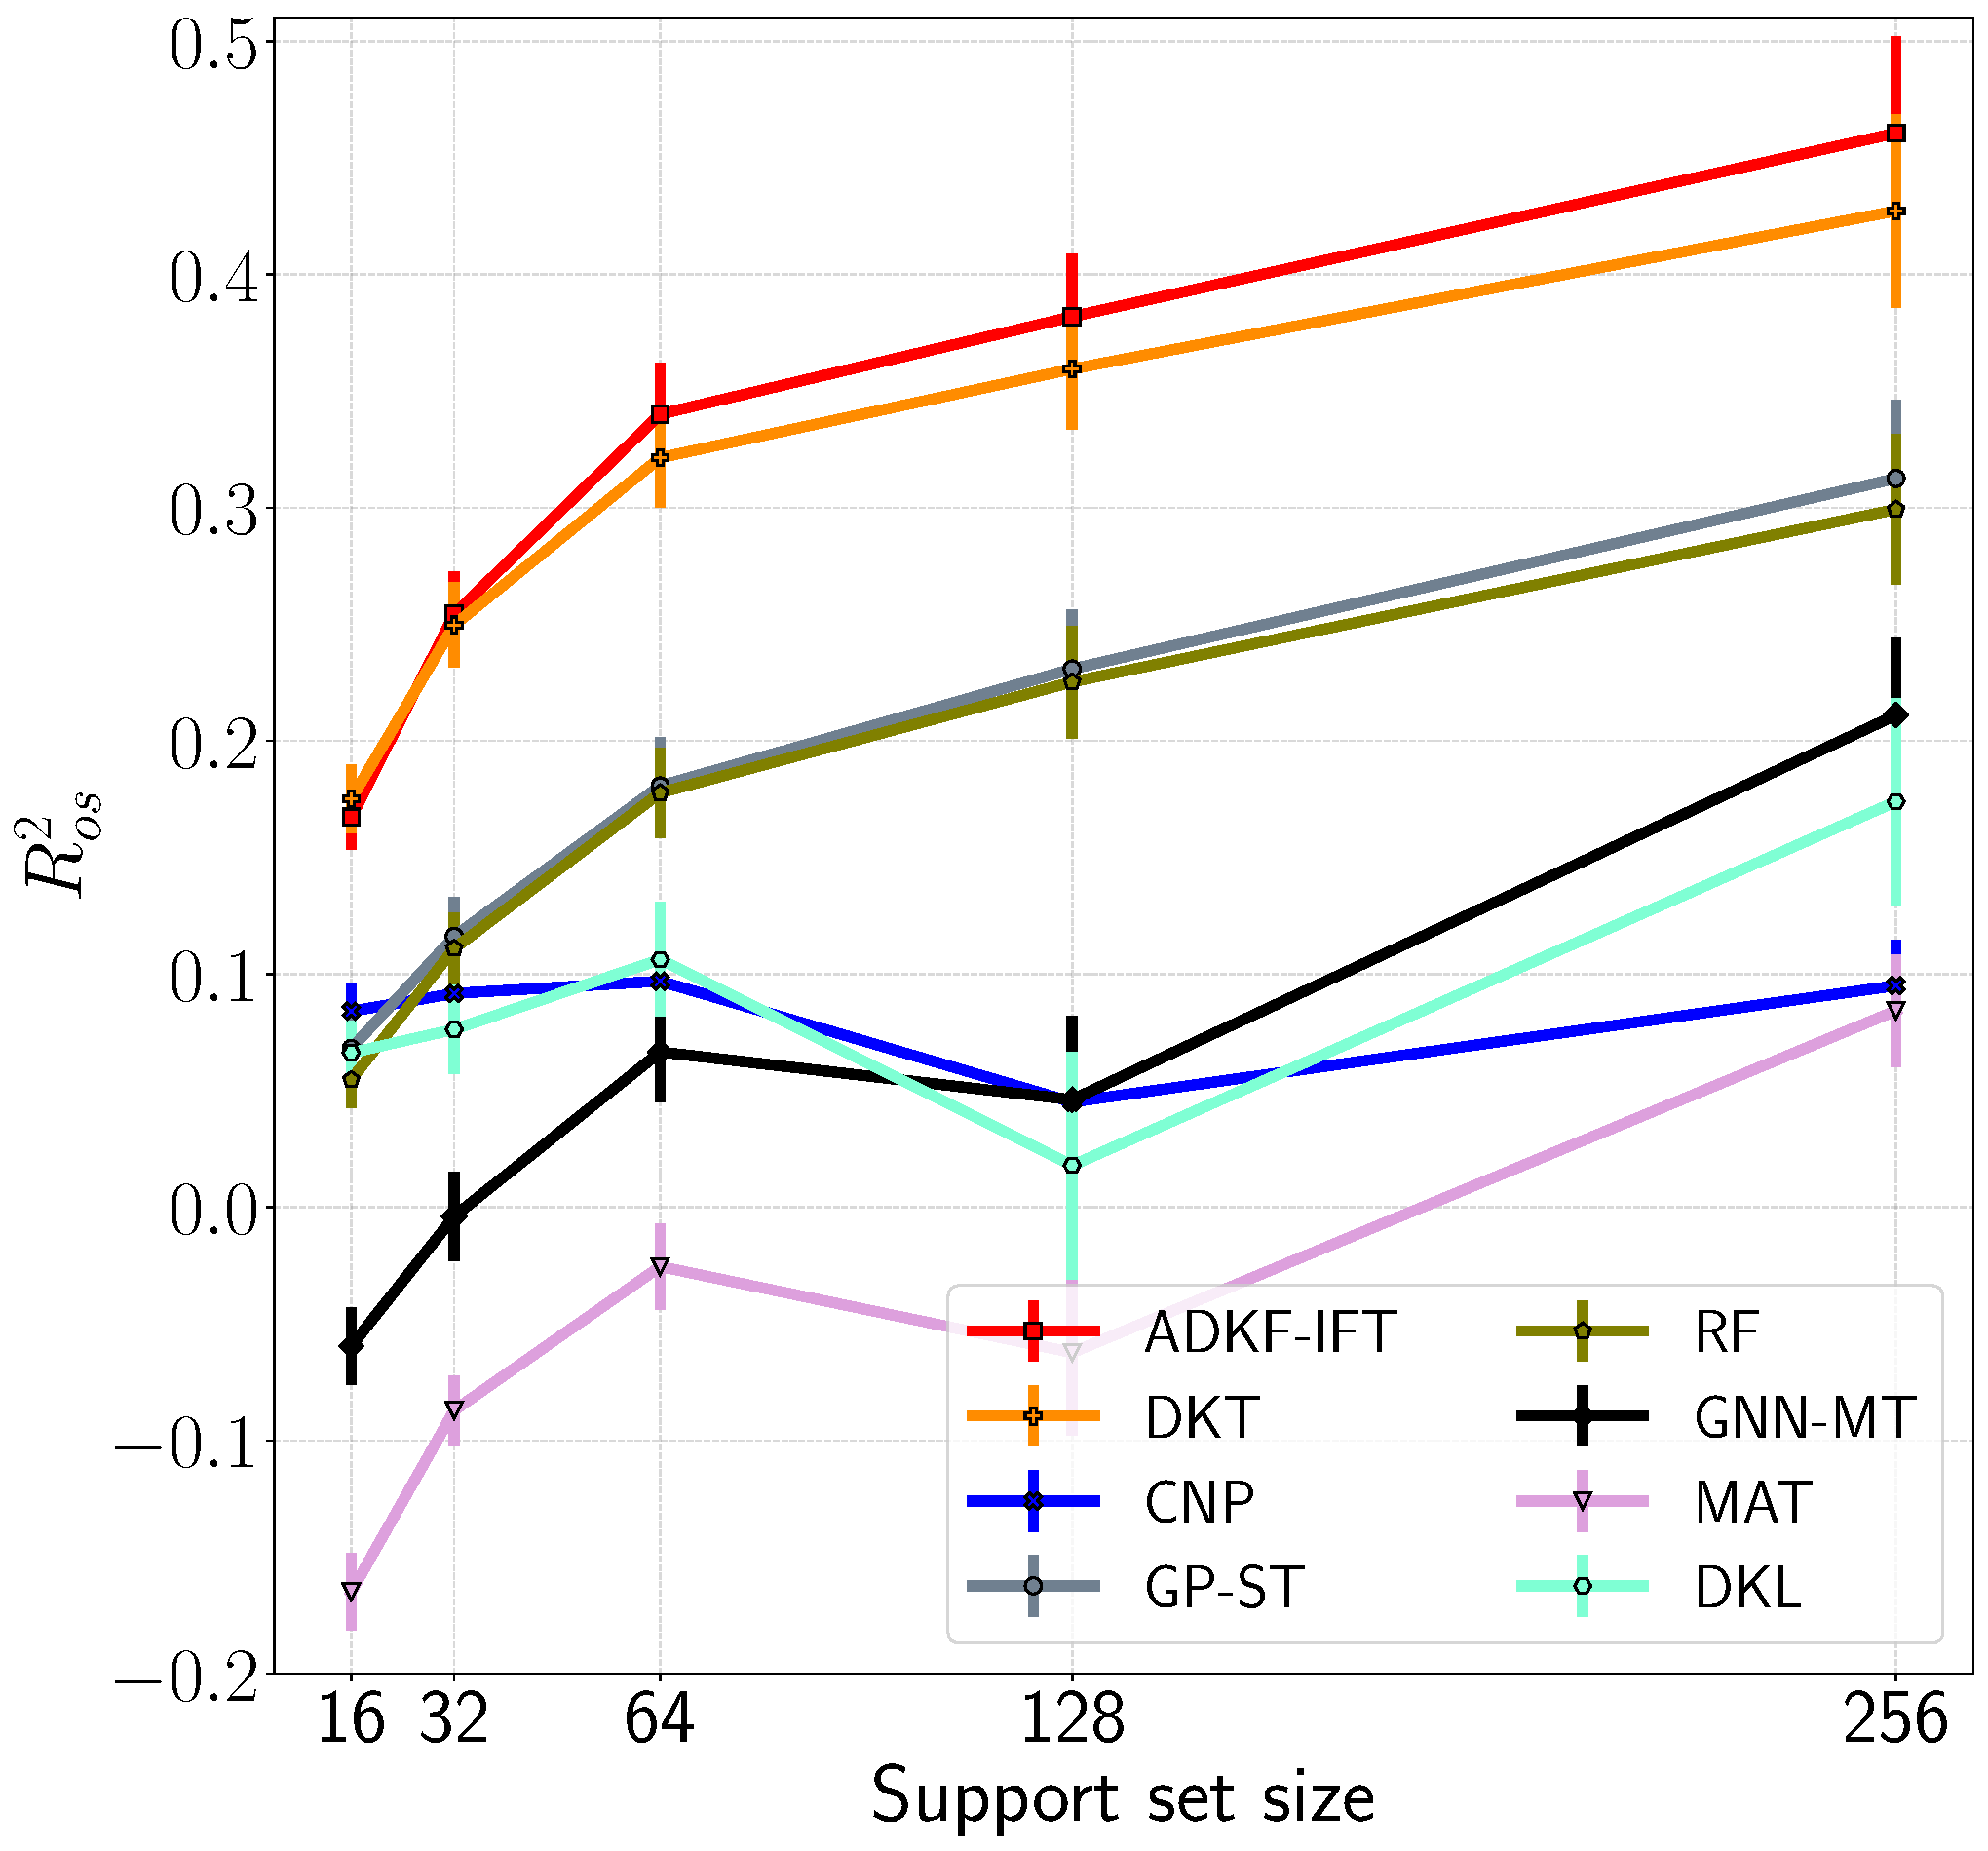
\includegraphics[width=\textwidth]{comparison_plot_hc_all_numeric.pdf}
                \caption{Regression (111 tasks).}
            \end{subfigure}
        \caption{Mean performance with standard errors of all compared methods on all FS-Mol test tasks.}
        \label{fig:aggregated-perforamnce}
        \end{figure}
        Figure~\ref{fig:aggregated-perforamnce} shows the overall test performance of all compared methods.
        Note that RF is 
        a strong baseline method, as it is widely used in real-world drug discovery projects
        and has comparable performance to 
        many %
        pretraining methods.
        The results indicate that ADKF-IFT outperforms all the other compared methods at all
        considered support set sizes for the classification task.
        For the regression task, the performance gains of ADKF-IFT over the second-best method,
        namely DKT, get larger as the support set size increases.

        Because mean performance can be influenced by outliers, in
        Table~\ref{tab:ranking} we plot the mean rank of all methods across all tasks.
        ADKF-IFT achieves the best mean rank for both classification and regression tasks
        at all considered support set sizes. The trends of these mean ranks are consistent to
        those in Figure \ref{fig:aggregated-perforamnce}.

        \begin{table}
            \scriptsize
            \caption{{\color{black}Mean ranks of all compared methods in terms of their performance on all FS-Mol test tasks.}}
            \label{tab:ranking}
            \begin{subtable}{.49\linewidth}
                \caption{Classification (157 tasks).}
                \centering
                \setlength\extrarowheight{-3pt}
                \begin{tabular}{cccccc}
                    \toprule
                    \multirow{2}[3]{*}{Method} & \multicolumn{5}{c}{Support set size}\\
                    \cmidrule(lr){2-6}
                    & 16 & 32 & 64 & 128 & 256 \\
                    \midrule
                    GNN-ST & $11.29$ & $11.53$ & $11.75$ & $11.85$ & $12.19$ \\
                    kNN & $10.89$ & $10.48$ & $10.33$ & $10.15$ & $9.37$ \\
                    MAT & $10.43$ & $10.44$ & $10.19$ & $9.69$ & $9.70$ \\
                    RF & $8.15$ & $7.89$ & $7.06$ & $6.25$ & $4.47$ \\
                    PAR & $7.70$ & $7.98$ & $8.30$ & $8.83$ & $10.81$ \\
                    GNN-MT & $7.33$ & $7.18$ & $7.08$ & $6.59$ & $6.53$ \\
                    DKL & $7.28$ & $7.49$ & $7.98$ & $8.42$ & $8.21$ \\
                    GP-ST & $6.71$ & $6.57$ & $6.28$ & $6.18$ & $5.14$ \\
                    GNN-MAML & $6.36$ & $6.92$ & $7.42$ & $7.89$ & $8.90$ \\
                    CNP & $5.00$ & $5.81$ & $6.36$ & $6.91$ & $7.78$ \\ 
                    ProtoNet & $4.00$ & $3.40$ & $3.11$ & $2.98$ & $3.85$ \\
                    DKT & $3.44$ & $3.19$ & $2.99$ & $2.99$ & $2.67$ \\
                    ADKF-IFT & $\mathbf{2.41}$ & $\mathbf{2.12}$ & $\mathbf{2.14}$ & $\mathbf{2.26}$ & $\mathbf{1.38}$ \\
                    \bottomrule
                \end{tabular}
            \end{subtable}
            \hfill
            \begin{subtable}{.49\linewidth}
                \caption{Regression (111 tasks).}
                \centering
                \begin{tabular}{cccccc}
                    \toprule
                    \multirow{2}[3]{*}{Method} & \multicolumn{5}{c}{Support set size}\\
                    \cmidrule(lr){2-6}
                    & 16 & 32 & 64 & 128 & 256 \\
                    \midrule
                    MAT & $7.60$ & $7.45$ & $7.26$ & $7.06$ & $7.19$ \\
                    GNN-MT & $6.61$ & $6.40$ & $6.15$ & $5.95$ & $5.58$ \\
                    RF & $5.00$ & $4.47$ & $4.16$ & $3.72$ & $3.56$ \\
                    DKL & $4.42$ & $5.16$ & $5.63$ & $6.10$ & $6.35$ \\
                    GP-ST & $4.23$ & $4.14$ & $3.87$ & $3.37$ & $3.07$ \\
                    CNP & $3.88$ & $4.45$ & $4.95$ & $5.73$ & $6.47$ \\
                    DKT & $\mathbf{2.12}$ & $2.08$ & $2.29$ & $2.32$ & $2.43$ \\
                    ADKF-IFT & $\mathbf{2.12}$ & $\mathbf{1.86}$ & $\mathbf{1.68}$ & $\mathbf{1.74}$ & $\mathbf{1.36}$ \\
                    \bottomrule
                \end{tabular}
            \end{subtable}
        \end{table}
        
        \subsubsection{Statistical Comparison}
        \begin{table}[ht]
            \tiny
            \caption[Results of Wilcoxon signed-rank test for ADKF-IFT's performance.]{$p$-values from the two-sided Wilcoxon signed-rank test for statistical comparisons between ADKF-IFT and DKT/DKT$+$/ADKF. The null hypothesis is that the median of their performance differences on all FS-Mol test tasks is zero. The significance level is set to $\alpha=0.05$.}
            \label{tab:statistical-comparisons}
            \centering
            \begin{tabular}{ccccccc}
                \toprule
                \multirow{2}[3]{*}{Compared models} & \multirow{2}[3]{*}{Task type} & \multicolumn{5}{c}{Support set size}\\
                \cmidrule(lr){3-7}
                & & 16 & 32 & 64 & 128 & 256 \\
                \midrule
                \multirow{2}[1]{*}{ADKF-IFT vs DKT} & Classification & $\;\:\mathbf{1.4\times10^{-12}}$ & $\;\:\mathbf{8.1\times10^{-14}}$ & $\:\,\mathbf{2.3\times10^{-12}}$ & $\mathbf{1.0\times10^{-8}}$ & $\mathbf{3.4\times10^{-7}}$ \\
                & Regression & $8.2\times10^{-2}$ & $9.6\times10^{-2}$ & $\mathbf{3.7\times10^{-5}}$ & $\mathbf{7.1\times10^{-5}}$ & $\mathbf{9.8\times10^{-7}}$ \\
                \midrule
                \multirow{2}[1]{*}{ADKF-IFT vs DKT$+$} & Classification & $\;\:\mathbf{3.2\times10^{-13}}$ & $\;\:\mathbf{7.0\times10^{-15}}$ & $\:\,\mathbf{2.3\times10^{-13}}$ & $\mathbf{1.2\times10^{-9}}$ & $\mathbf{1.6\times10^{-6}}$ \\
                & Regression & $\mathbf{3.2\times10^{-2}}$ & $4.2\times10^{-1}$ & $\mathbf{3.4\times10^{-5}}$ & $\:\:\mathbf{5.2\times10^{-10}}$ & $\mathbf{1.2\times10^{-5}}$ \\
                \midrule
                \multirow{2}[1]{*}{ADKF-IFT vs ADKF} & Classification & $\mathbf{1.7\times10^{-2}}$ & $1.1\times10^{-1}$ & $4.8\times10^{-1}$ & $8.3\times10^{-1}$ & $\mathbf{1.6\times10^{-3}}$ \\
                & Regression & $\mathbf{2.8\times10^{-3}}$ & $\mathbf{4.2\times10^{-4}}$ & $\mathbf{1.3\times10^{-3}}$ & $\mathbf{4.1\times10^{-6}}$ & $\mathbf{1.3\times10^{-5}}$ \\
                \bottomrule
            \end{tabular}
        \end{table}
        Table \ref{tab:statistical-comparisons} shows the $p$-values from a two-sided Wilcoxon signed-rank test for statistical comparisons between ADKF-IFT and the next second method, namely DKT.
        The test results indicate that their median performance difference is non-zero
        (i.e., ADKF-IFT significantly outperforms DKT) for the classification task at all considered support
        set sizes and for the regression task at support set sizes 64, 128, and 256
        (at significance level $\alpha=0.05$).
        The $p$-values for statistical comparisons between ADKF-IFT and the two ablation models
        DKT$+$ and ADKF are also shown in Table~\ref{tab:statistical-comparisons},
        demonstrating that ADKF-IFT significantly outperforms these ablation models in most cases.
        
        \subsubsection{Ablation Study}
        \begin{figure}[ht]
            \centering
            \begin{subfigure}{.45\textwidth}
                \centering
                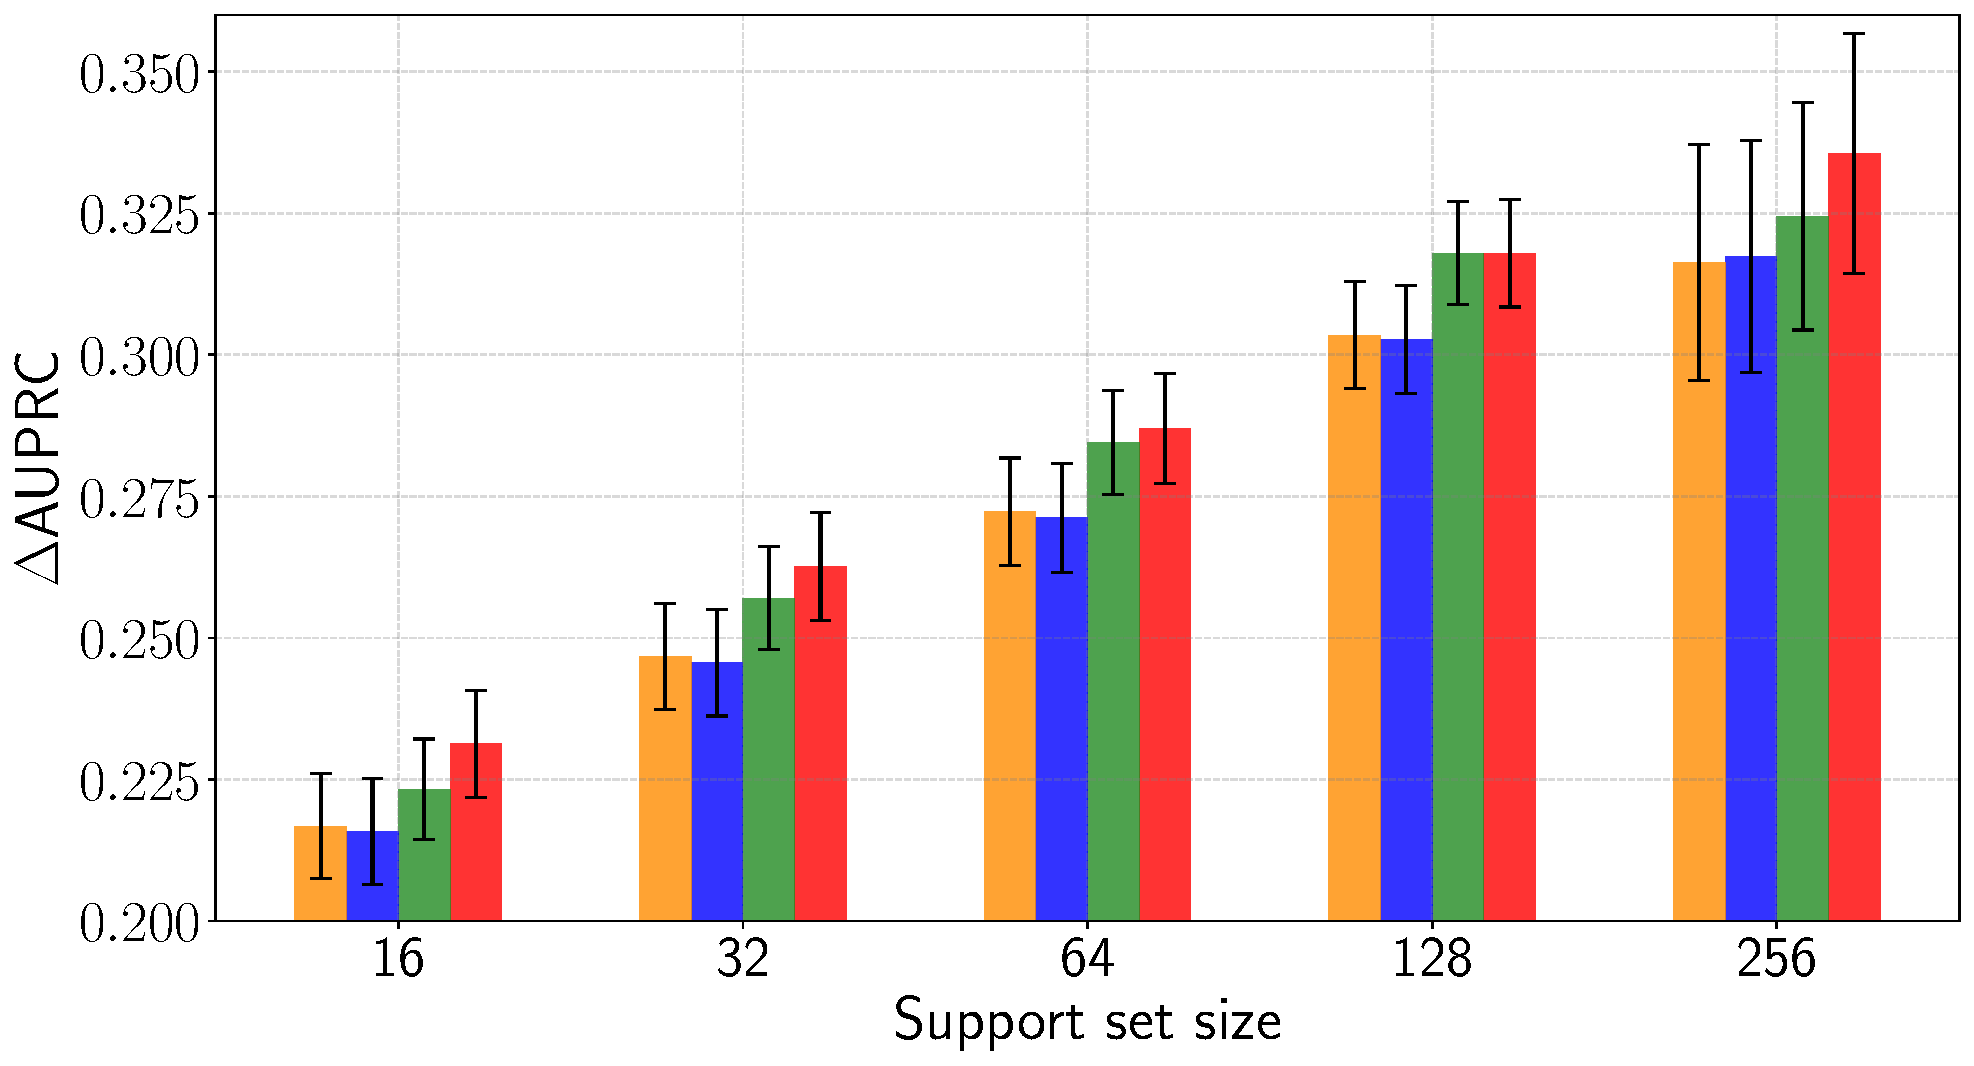
\includegraphics[width=\textwidth]{comparison_plot_hc_all_ablation.pdf}
                \caption{Classification (157 tasks).}
            \end{subfigure}
            \hfill
            \begin{subfigure}{.45\textwidth}
                \centering
                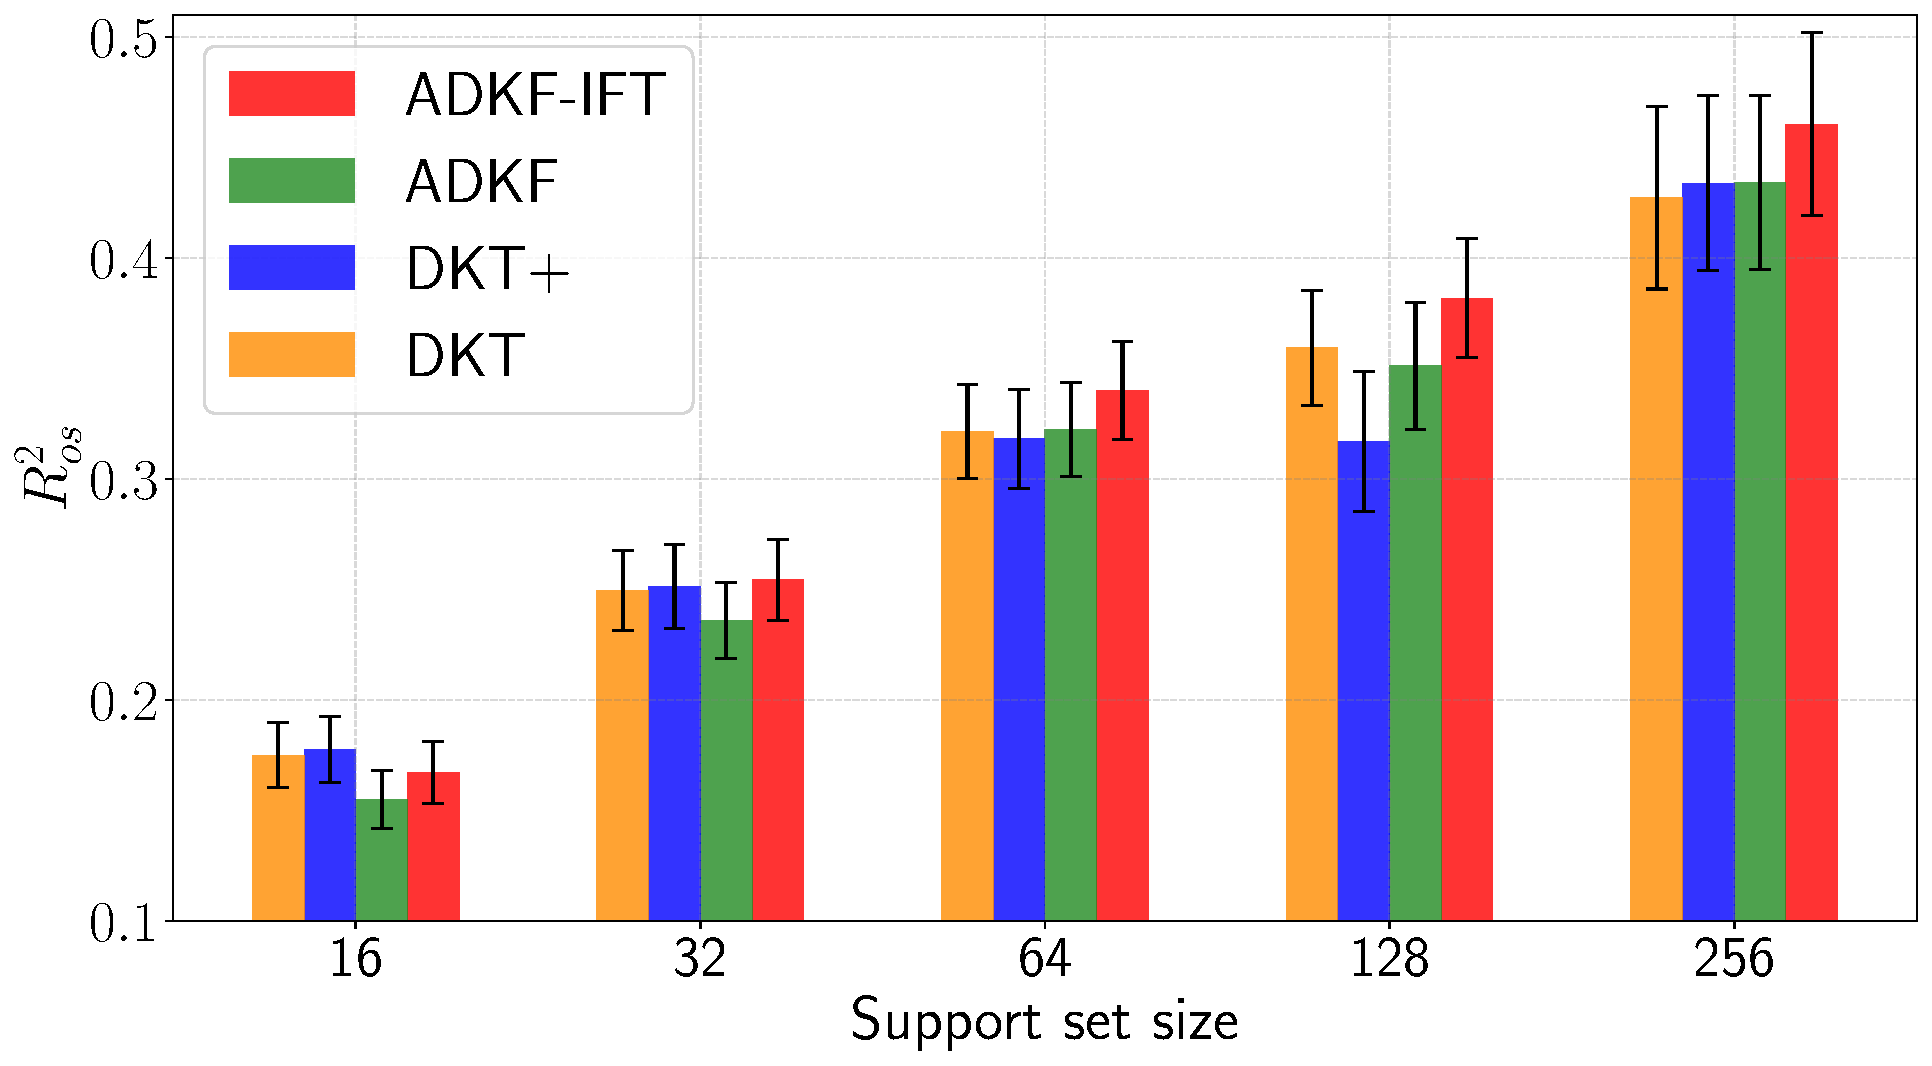
\includegraphics[width=\textwidth]{comparison_plot_hc_all_ablation_numeric.pdf}
                \caption{Regression (111 tasks).}
            \end{subfigure}
            \caption[Ablation study results on FS-Mol.]{Mean performance with standard errors of ablation models on all FS-Mol test tasks. ADKF is like ADKF-IFT but assuming $\nicefrac{\partial\bftheta^*}{\partial\bfphi}=\bfzero$, i.e., updating $\bfphi$ with the direct gradient $\nicefrac{\partial \loss_V}{\partial\bfphi}$. DKT$+$ is like DKT but tuning the base kernel parameters $\bftheta$ during meta-testing.}
            \label{fig:ablation-study}
        \end{figure}
        To show that 1) the bilevel optimisation objective for ADKF-IFT is essential for
        learning informative feature representations and 2) the performance gains of ADKF-IFT
        are not simply caused by tuning the base kernel parameters $\bftheta$ at meta-test time,
        we consider two ablation models: DKT$+$ and ADKF. The test performance of these models are
        shown in Figure \ref{fig:ablation-study}. For ADKF, we follow the ADKF-IFT training scheme
        but assume $\nicefrac{\partial\bftheta^*}{\partial\bfphi}=\bfzero$, i.e., updating the feature
        extractor parameters $\bfphi$ with the \emph{direct gradient}
        $\nicefrac{\partial \loss_V}{\partial\bfphi}$ rather than $\nicefrac{d\loss_V}{d\bfphi}$.
        The results show that ADKF consistently underperforms ADKF-IFT, indicating that the
        hypergradient for the bilevel optimisation objective has non-negligible contributions
        to learning better feature representations. For DKT$+$, we take a model trained by DKT
        and adapt the base kernel parameters $\bftheta$ on each task at meta-test time.
        The results show that DKT$+$ does not improve upon DKT, indicating that tuning the
        base kernel parameters $\bftheta$ at meta-test time is not sufficient for obtaining
        better test performance with DKT.
        
        \subsubsection{Sub-benchmark Performance}
        The tasks in FS-Mol can be partitioned into 7 sub-benchmarks by Enzyme Commission number
        \citep{Webb92enzymenomenclature}.
        Ideally, the best method should be able to perform well across all sub-benchmarks.
        Table~\ref{tab:sub-benchmark} shows the test performance of top performing methods
        on all sub-benchmarks at support set size 64 (the median of all considered support sizes)
        for both the classification and regression tasks. The results indicate that,
        in addition to achieving the best overall performance, ADKF-IFT achieves the best performance
        on all sub-benchmarks for the regression task and on more than half of the sub-benchmarks
        for the classification task.
        \begin{table}[ht]
            \tiny
            \caption[Sub-benchmark results on FS-Mol.]{Mean performance with standard errors of top performing methods on FS-Mol test tasks within each sub-benchmark (broken down by EC category) at support set size 64 (the median of all considered support sizes). Note that class 2 is most common in the FS-Mol training set ($\sim 1,500$ training tasks), whereas classes 6 and 7 are least common in the FS-Mol training set ($<50$ training tasks each).}
            \label{tab:sub-benchmark}
            \begin{subtable}{1.0\linewidth}
                \caption{Classification ($\Delta$AUPRC).}
                \centering
                \begin{tabular}{cccccccc}
                \toprule
                \multicolumn{3}{c}{FS-Mol sub-benchmark (EC category)} & \multicolumn{5}{c}{Method} \\
                \cmidrule(lr){1-3}\cmidrule(lr){4-8}
                Class & Description & \#tasks & RF & GP-ST & ProtoNet & DKT & ADKF-IFT \\
                \midrule
                1 & oxidoreductases & 7 & $0.156\pm 0.044$ & $0.152\pm 0.040$ & $0.137\pm 0.037$ & $0.145\pm 0.040$ & $\mathbf{0.160\pm 0.045}$ \\
                2 & kinases & 125 & $0.152\pm 0.009$ & $0.161\pm 0.009$ & $0.285\pm 0.010$ & $0.282\pm 0.010$ & $\mathbf{0.299\pm 0.010}$ \\
                3 & hydrolases & 20 & $0.229\pm 0.032$ & $0.230\pm 0.032$ & $0.245\pm 0.034$ & $0.254\pm 0.034$ & $\mathbf{0.262\pm 0.033}$ \\
                4 & lysases & 2 & $0.276\pm 0.182$ & $\mathbf{0.284\pm 0.189}$ & $0.265\pm 0.211$ & $0.272\pm 0.206$ & $0.279\pm 0.201$ \\
                5 & isomerases & 1 & $0.166\pm 0.040$ & $\mathbf{0.212\pm 0.052}$ & $0.172\pm 0.044$ & $0.204\pm 0.058$ & $0.198\pm 0.046$ \\
                6 & ligases & 1 & $0.149\pm 0.035$ & $0.199\pm 0.028$ & $0.170\pm 0.028$ & $0.229\pm 0.013$ & $\mathbf{0.231\pm 0.022}$ \\
                7 & translocases & 1 & $\mathbf{0.128\pm 0.039}$ & $0.109\pm 0.049$ & $0.099\pm 0.028$ & $0.122\pm 0.022$ & $0.109\pm 0.033$ \\
                \midrule
                & all enzymes & 157 & $0.163\pm 0.009$ & $0.171\pm 0.009$ & $0.271\pm 0.009$ & $0.271\pm 0.010$ & $\mathbf{0.285\pm 0.010}$ \\
                \bottomrule
            \end{tabular}
            \end{subtable}
            
            \begin{subtable}{1.0\linewidth}
                \caption{Regression ($R_{os}^2$).}
                \centering
                \begin{tabular}{cccccccc}
                \toprule
                \multicolumn{3}{c}{FS-Mol sub-benchmark (EC category)} & \multicolumn{5}{c}{Method} \\
                \cmidrule(lr){1-3}\cmidrule(lr){4-8}
                Class & Description & \#tasks & RF & GP-ST & CNP & DKT & ADKF-IFT \\
                \midrule
                1 & oxidoreductases & 6 & $0.108\pm 0.087$ & $0.103\pm 0.076$ & $-0.012\pm 0.011$ & $0.098\pm 0.078$ & $\mathbf{0.116\pm 0.079}$ \\
                2 & kinases & 82 & $0.160\pm 0.019$ & $0.162\pm 0.022$ & $\:\:\,\,0.127\pm 0.017$ & $0.343\pm 0.022$ & $\mathbf{0.363\pm 0.024}$ \\
                3 & hydrolases & 19 & $0.256\pm 0.058$ & $0.267\pm 0.061$ & $\:\:\,\,0.014\pm 0.015$ & $0.295\pm 0.063$ & $\mathbf{0.310\pm 0.062}$ \\
                4 & lysases & 2 & $0.418\pm 0.405$ & $0.417\pm 0.416$ & $\:\:\,\,0.100\pm 0.068$ & $0.440\pm 0.418$ & $\mathbf{0.442\pm 0.403}$ \\
                5 & isomerases & 1 & $0.125\pm 0.077$ & $0.086\pm 0.082$ & $-0.012\pm 0.010$ & $0.209\pm 0.113$ & $\mathbf{0.226\pm 0.063}$ \\
                6 & ligases & 1 & $0.182\pm 0.040$ & $0.202\pm 0.079$ & $\:\:\,\,0.002\pm 0.004$ & $0.277\pm 0.035$ & $\mathbf{0.279\pm 0.043}$ \\
                7 & translocases & 0 & N/A & N/A & N/A & N/A & N/A \\
                \midrule
                & all enzymes & 111 & $0.178\pm 0.019$ & $0.181\pm 0.021$ & $\:\:\,\,0.097\pm 0.014$ & $0.321\pm 0.021$ & $\mathbf{0.340\pm 0.022}$ \\
                \bottomrule
            \end{tabular}
            \end{subtable}
        \end{table}
        
        
    
    \subsection{Out-of-domain Molecular Property Prediction and optimisation}\label{sec:adkf:mol-opt}
        Finally, we demonstrate that the feature representation learned by ADKF-IFT is useful not only for
        in-domain molecular property prediction tasks but also for out-of-domain molecular property
        prediction and optimisation tasks. For this, we perform experiments involving finding molecules
        with best desired target properties within given out-of-domain datasets using
        Bayesian optimisation (BO) with a GP surrogate model operating on top of compared
        feature representations. We use the expected improvement acquisition function \citep{jones1998efficient}
        with query-batch size 1. All compared feature representations are extracted using the models
        trained on the FS-Mol dataset from scratch in Section~\ref{sec:few-shot-experiments},
        except for the pretrained MAT representation and fingerprint. We compare them
        on four representative molecular design tasks outside of FS-Mol.

        \subsubsection{Description of Tasks}

        \begin{table}[ht]
            \tiny
            \caption{Descriptions of four out-of-domain molecular design tasks.}
            \label{tab:optimisation tasks}
            \centering
            \begin{tabular}{ccccc}
                \toprule
                Molecular design task & Data source & \#compounds & Target & Target source \\
                \midrule
                Molecular docking (ESR2) & \textsc{DockString} training set & 2,312 & binding score & AutoDock Vina \\
                Antibiotic discovery (E. coli BW25113) & Antibiotic training set & 2,335 & relative growth & screening\\
                Antiviral drug design (SARS-CoV-2) & COVID Moonshot & 1,926 & pIC50 Fluorescence & experimental lab \\
                Material design (Organic Photovoltaic) & Harvard Clean Energy Project & 2,012 & power conversion efficiency & DFT simulation \\
                \bottomrule
            \end{tabular}
        \end{table}

        Table~\ref{tab:optimisation tasks} summarizes the datasets considered.
        Note that the datasets for the molecular
        docking and material design tasks are subsampled from the much larger datasets provided
        in \textsc{DockString} \citep{ortegon2021dockstring} and Harvard Clean Energy Project
        \citep{hachmann2011harvard}, respectively. The datasets for the antibiotic discovery
        and antiviral drug design tasks are taken from the antibiotic training set and the
        COVID Moonshot dataset provided in \citet{STOKES2020} and \citet{covidmoonshot},
        respectively. We repeat each BO experiment 20 times, each time starting from 16
        randomly sampled molecules from the worst $\sim 700$ molecules within the dataset. 
        
        The ``fingerprint'' GP baseline
        uses the Tanimoto kernel on
        2048 dimensional count Morgan fingerprints of radius 2 (defined in \S\ref{definition:morgan-fingerprint}).
        All other baseline feature representations use the Mat\'ern52 kernel
        without ARD (with a log-normal prior over the lengthscale, centered at the
        median heuristic initialization).
        We re-fit the base kernel parameters using all available data points at the beginning
        of each BO iteration.

        \subsubsection{Results}

        Figure \ref{fig:bo} shows that the ADKF-IFT representation enables the fastest discovery of
        top performing molecules for the molecular docking, antibiotic discovery, and material design tasks. For the antiviral
        drug design task, although the ADKF-IFT representation underperforms the MAT and GNN-MT representations, it still achieves
        competitive performance compared to other baselines.
        
        Table \ref{tab:bo-predictive} explicitly reports the regression predictive performance of a GP operating on top of
        each compared feature representation for these four out-of-domain molecular design tasks. The configuration of the GP
        is the same as that in the BO experiments. We report test negative log likelihood (NLL) averaged over 200 support/query
        random splits (100 for each of the support set sizes 32 and 64). The results show that the ADKF-IFT representation has
        the best test NLL on the molecular docking, antibiotic discovery, and material design tasks, and ranks second on
        the antiviral drug design task.
        
        \begin{figure}[ht]
        \begin{subfigure}{.24\textwidth}
            \centering
            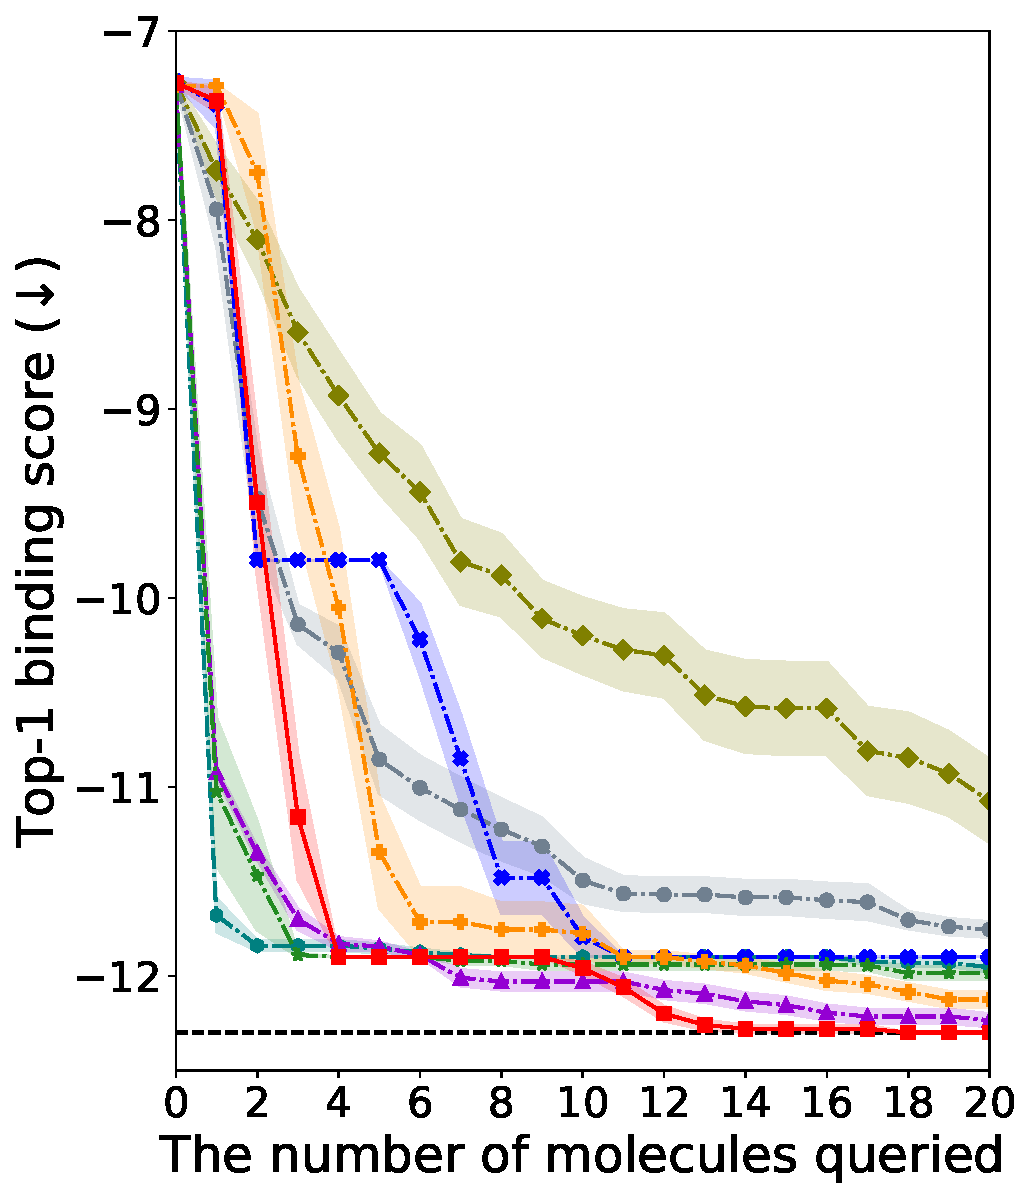
\includegraphics[width=\textwidth]{BO-dockstring.pdf}
            \caption{Molecular docking}
            \label{fig:bo-docking}
        \end{subfigure}
        \hfill
        \begin{subfigure}{.24\textwidth}
            \centering
            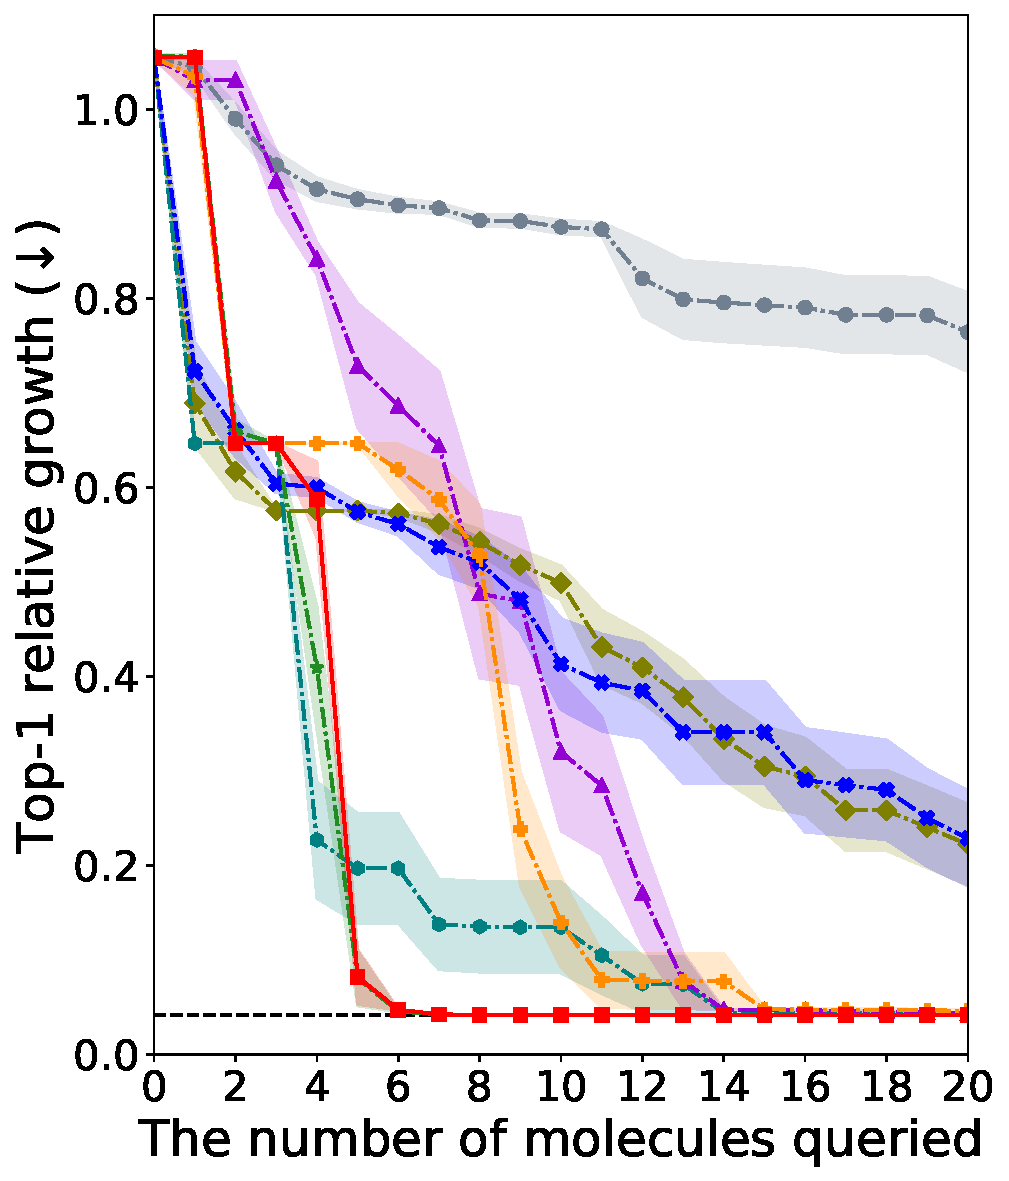
\includegraphics[width=\textwidth]{BO-antibiotics.pdf}
            \caption{Antibiotic discovery}
            \label{fig:bo-antibiotic}
        \end{subfigure}
        \begin{subfigure}{.24\textwidth}
            \centering
            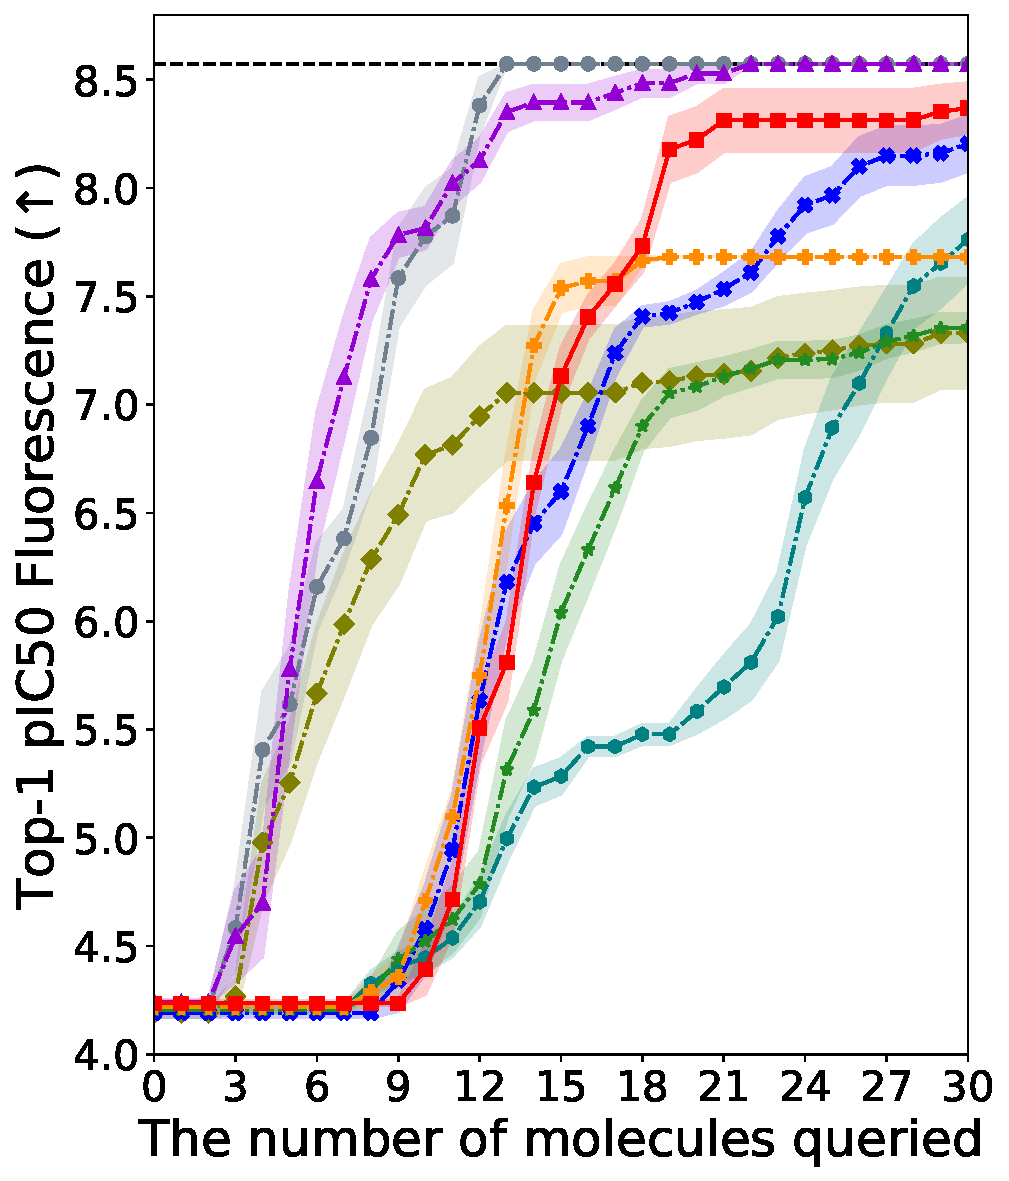
\includegraphics[width=\textwidth]{BO-covid.pdf}
            \caption{Antiviral design}  %
            \label{fig:bo-covid}
        \end{subfigure}
        \hfill
        \begin{subfigure}{.24\textwidth}
            \centering
            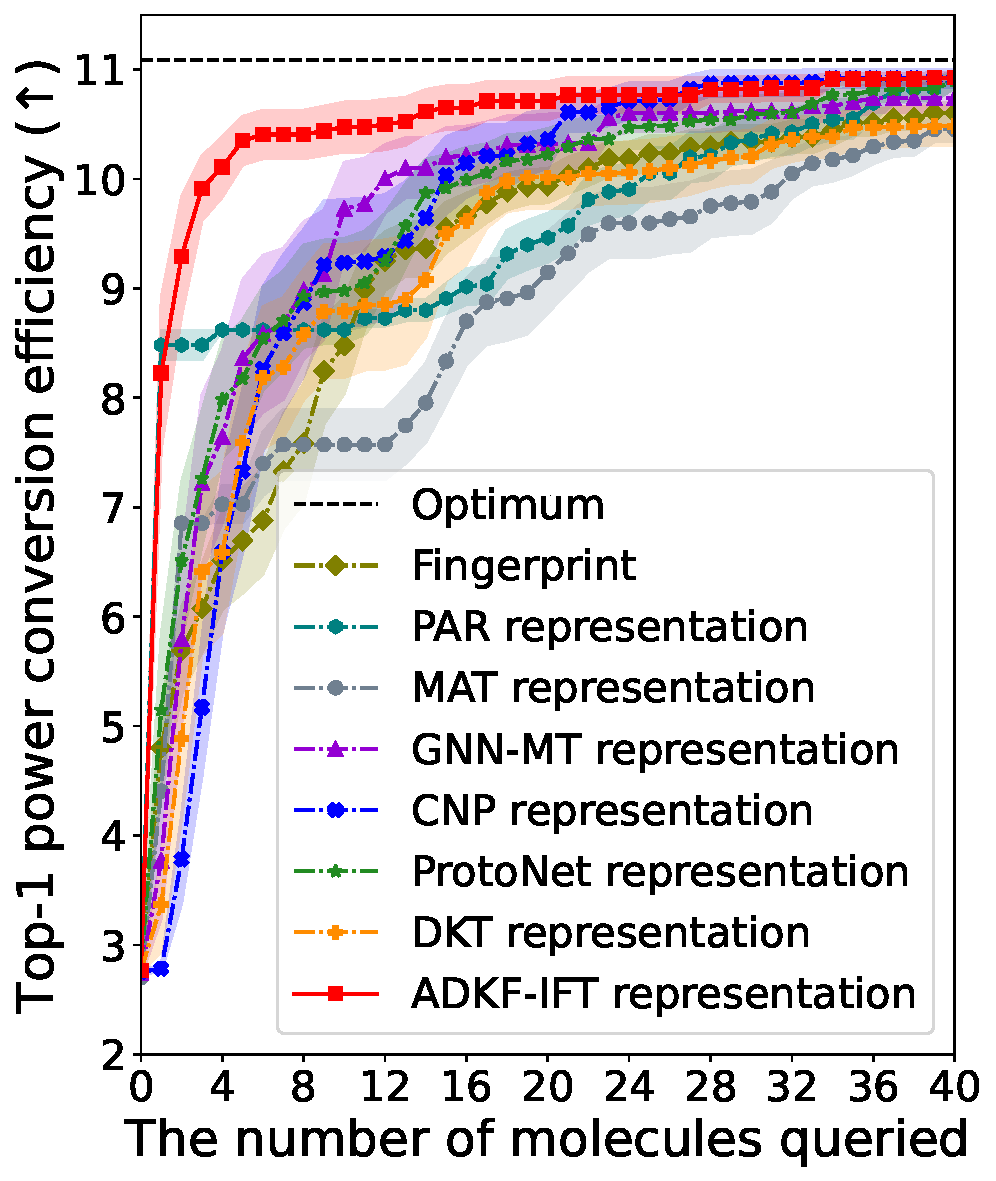
\includegraphics[width=\textwidth]{BO-opv.pdf}
            \caption{Material design}
            \label{fig:bo-opv}
        \end{subfigure}
        \caption[Top-K scores on out-of-domain molecular design tasks.]{Mean top-1 target values with standard errors as a function of the number of molecules queried for all compared feature representations on four out-of-domain molecular optimisation tasks.}
        \label{fig:bo}
    \end{figure}
    
        \begin{table}
        \footnotesize
        \caption[Predictive performance on out-of-domain molecular design tasks.]{Mean predictive performance (test NLL) with standard errors of a GP operating on top of each compared feature representation on the four out-of-domain molecular design tasks.}
        \label{tab:bo-predictive}
            \centering
            \setlength\extrarowheight{-3pt}
            \begin{tabular}{ccccc}
                \toprule
                \multirow{3}{*}{\makecell{Feature \\ representation}} & \multicolumn{4}{c}{Out-of-domain molecular design task} \\
                \cmidrule(lr){2-5}
                 & Molecular docking & Antibiotic discovery & Antiviral drug design & Material design \\
                 \midrule
                Fingerprint & $1.138\pm0.014$ & $1.669\pm0.075$ & $\mathbf{4.601\pm0.086}$ & $1.091\pm0.011$ \\
                PAR & $1.270\pm0.019$ & $2.185\pm0.115$ & $4.840\pm0.086$ & $1.283\pm0.017$\\
                MAT & $1.528\pm0.028$ & $2.390\pm0.104$ & $4.797\pm0.088$ & $2.198\pm0.063$ \\
                GNN-MT & $1.994\pm0.050$ & $3.692\pm0.225$ & $6.399\pm0.181$ & $7.254\pm0.217$ \\
                CNP & $1.493\pm0.028$ & $2.537\pm0.162$ & $5.005\pm0.086$ & $1.741\pm0.043$ \\ 
                ProtoNet &  $1.147\pm0.013$ & $1.615\pm0.094$ & $5.060\pm0.086$ & $1.032\pm0.009$ \\
                DKT & $1.167\pm0.012$ & $1.602\pm0.073$ & $4.975\pm0.092$ & $1.026\pm0.009$ \\
                ADKF-IFT & $\mathbf{1.137\pm0.011}$ & $\mathbf{1.496\pm0.043}$ & $4.781\pm0.087$ & $\mathbf{0.996\pm0.007}$ \\
                \bottomrule
            \end{tabular}
    \end{table}
        


\section{Discussion}\label{sec:adkf:conclusion}

We have proposed Adaptive Deep Kernel Fitting with Implicit Function Theorem (ADKF-IFT),
a novel framework for fitting deep kernels that interpolates between meta-learning and conventional deep kernel learning.
ADKF-IFT meta-learns a feature extractor across tasks such that the task-specific GP models estimated on top of the
extracted feature representations can achieve the lowest possible prediction error on average.
ADKF-IFT is implemented by solving a bilevel optimisation objective via implicit differentiation.
We have shown that ADKF-IFT is a unifying framework containing DKL and DKT as special cases.
We have demonstrated that ADKF-IFT learns generally useful feature representations, achieving state-of-the-art performance
on a variety of real-world few-shot molecular property prediction tasks and on out-of-domain molecular property prediction
and optimisation tasks. We believe that ADKF-IFT could potentially be an important method to produce well-calibrated models
for fully-automated high-throughput experimentation in the future. 

Some directions for future work are as follows: 
\begin{enumerate}
    \item Using ARD in the base kernel so that feature selection for each individual task can be done by the GP model, with potential overfitting problems being reduced by assuming a sparse prior over lengthscales or by learning a low-dimensional manifold for them.
    \item Adapting the feature extractor to each task as well by allowing small deviations across tasks according to a meta-learned prior on the feature extractor parameters (e.g., as described in \citet{chen2020modular}).
    \item Adopting a more principled approximate inference strategy for few-shot GP classification (e.g., Pólya-Gamma data augmentation \citep{snell2020bayesian} or Laplace approximation \citep{kim2021gaussian}).
    \item Injecting domain expertise in drug discovery into the base kernel with hand-curated features and kernel combinations.
\end{enumerate}

\section{Retrospective}

Although this work was published fairly recently,
a small number of follow-up papers testing meta-learning methods on molecules
have shown that ADKF performs favourably
\citep{
    ortegon2024graph,  %
    schimunek2023contextenriched%
}.
Therefore, I am optimistic that ADKF will at least be tried by chemists at some point in the future.
However, I think ADKF's practical performance will be limited in the long term
by the availability of meta-datasets for training the feature extractor.
Follow-up work by \citet{klarner2022bias} has shown that popular meta-learning datasets
contain a lot of ``false positive'' molecules, effectively making them very noisy.
Although future datasets could overcome this, for meta-learning to make sense the different tasks
in the meta-dataset should ideally be related to each other in some way,
otherwise the feature extractor will not be able to learn anything useful
(beyond a low-dimensional representation of the input space).
In this setting, I am unsure whether a deep kernel would perform better than a simple graph kernel.
It was this uncertainty which led me to re-examine simpler graph kernels,
leading to the contributions of the next chapter.
